\documentclass[twoside]{book}

% Packages required by doxygen
\usepackage{fixltx2e}
\usepackage{calc}
\usepackage{doxygen}
\usepackage[export]{adjustbox} % also loads graphicx
\usepackage{graphicx}
\usepackage[utf8]{inputenc}
\usepackage{makeidx}
\usepackage{multicol}
\usepackage{multirow}
\PassOptionsToPackage{warn}{textcomp}
\usepackage{textcomp}
\usepackage[nointegrals]{wasysym}
\usepackage[table]{xcolor}

% Font selection
\usepackage[T1]{fontenc}
\usepackage[scaled=.90]{helvet}
\usepackage{courier}
\usepackage{amssymb}
\usepackage{sectsty}
\renewcommand{\familydefault}{\sfdefault}
\allsectionsfont{%
  \fontseries{bc}\selectfont%
  \color{darkgray}%
}
\renewcommand{\DoxyLabelFont}{%
  \fontseries{bc}\selectfont%
  \color{darkgray}%
}
\newcommand{\+}{\discretionary{\mbox{\scriptsize$\hookleftarrow$}}{}{}}

% Page & text layout
\usepackage{geometry}
\geometry{%
  a4paper,%
  top=2.5cm,%
  bottom=2.5cm,%
  left=2.5cm,%
  right=2.5cm%
}
\tolerance=750
\hfuzz=15pt
\hbadness=750
\setlength{\emergencystretch}{15pt}
\setlength{\parindent}{0cm}
\setlength{\parskip}{3ex plus 2ex minus 2ex}
\makeatletter
\renewcommand{\paragraph}{%
  \@startsection{paragraph}{4}{0ex}{-1.0ex}{1.0ex}{%
    \normalfont\normalsize\bfseries\SS@parafont%
  }%
}
\renewcommand{\subparagraph}{%
  \@startsection{subparagraph}{5}{0ex}{-1.0ex}{1.0ex}{%
    \normalfont\normalsize\bfseries\SS@subparafont%
  }%
}
\makeatother

% Headers & footers
\usepackage{fancyhdr}
\pagestyle{fancyplain}
\fancyhead[LE]{\fancyplain{}{\bfseries\thepage}}
\fancyhead[CE]{\fancyplain{}{}}
\fancyhead[RE]{\fancyplain{}{\bfseries\leftmark}}
\fancyhead[LO]{\fancyplain{}{\bfseries\rightmark}}
\fancyhead[CO]{\fancyplain{}{}}
\fancyhead[RO]{\fancyplain{}{\bfseries\thepage}}
\fancyfoot[LE]{\fancyplain{}{}}
\fancyfoot[CE]{\fancyplain{}{}}
\fancyfoot[RE]{\fancyplain{}{\bfseries\scriptsize Generated by Doxygen }}
\fancyfoot[LO]{\fancyplain{}{\bfseries\scriptsize Generated by Doxygen }}
\fancyfoot[CO]{\fancyplain{}{}}
\fancyfoot[RO]{\fancyplain{}{}}
\renewcommand{\footrulewidth}{0.4pt}
\renewcommand{\chaptermark}[1]{%
  \markboth{#1}{}%
}
\renewcommand{\sectionmark}[1]{%
  \markright{\thesection\ #1}%
}

% Indices & bibliography
\usepackage{natbib}
\usepackage[titles]{tocloft}
\setcounter{tocdepth}{3}
\setcounter{secnumdepth}{5}
\makeindex

% Hyperlinks (required, but should be loaded last)
\usepackage{ifpdf}
\ifpdf
  \usepackage[pdftex,pagebackref=true]{hyperref}
\else
  \usepackage[ps2pdf,pagebackref=true]{hyperref}
\fi
\hypersetup{%
  colorlinks=true,%
  linkcolor=blue,%
  citecolor=blue,%
  unicode%
}

% Custom commands
\newcommand{\clearemptydoublepage}{%
  \newpage{\pagestyle{empty}\cleardoublepage}%
}

\usepackage{caption}
\captionsetup{labelsep=space,justification=centering,font={bf},singlelinecheck=off,skip=4pt,position=top}

%===== C O N T E N T S =====

\begin{document}

% Titlepage & ToC
\hypersetup{pageanchor=false,
             bookmarksnumbered=true,
             pdfencoding=unicode
            }
\pagenumbering{alph}
\begin{titlepage}
\vspace*{7cm}
\begin{center}%
{\Large My Project }\\
\vspace*{1cm}
{\large Generated by Doxygen 1.8.13}\\
\end{center}
\end{titlepage}
\clearemptydoublepage
\pagenumbering{roman}
\tableofcontents
\clearemptydoublepage
\pagenumbering{arabic}
\hypersetup{pageanchor=true}

%--- Begin generated contents ---
\chapter{Hierarchical Index}
\section{Class Hierarchy}
This inheritance list is sorted roughly, but not completely, alphabetically\+:\begin{DoxyCompactList}
\item \contentsline{section}{Avaliation}{\pageref{class_avaliation}}{}
\item \contentsline{section}{Blog}{\pageref{class_blog}}{}
\item \contentsline{section}{Content}{\pageref{class_content}}{}
\begin{DoxyCompactList}
\item \contentsline{section}{Comment}{\pageref{class_comment}}{}
\item \contentsline{section}{Post}{\pageref{class_post}}{}
\end{DoxyCompactList}
\item \contentsline{section}{Domain}{\pageref{class_domain}}{}
\begin{DoxyCompactList}
\item \contentsline{section}{Email}{\pageref{class_email}}{}
\item \contentsline{section}{Name}{\pageref{class_name}}{}
\item \contentsline{section}{Password}{\pageref{class_password}}{}
\item \contentsline{section}{Text}{\pageref{class_text}}{}
\end{DoxyCompactList}
\item \contentsline{section}{Test\+Avaliation}{\pageref{class_test_avaliation}}{}
\item \contentsline{section}{Test\+Blog}{\pageref{class_test_blog}}{}
\item \contentsline{section}{Test\+Comment}{\pageref{class_test_comment}}{}
\item \contentsline{section}{Test\+Domain}{\pageref{class_test_domain}}{}
\begin{DoxyCompactList}
\item \contentsline{section}{Test\+Email}{\pageref{class_test_email}}{}
\item \contentsline{section}{Test\+Name}{\pageref{class_test_name}}{}
\item \contentsline{section}{Test\+Password}{\pageref{class_test_password}}{}
\item \contentsline{section}{Test\+Text}{\pageref{class_test_text}}{}
\end{DoxyCompactList}
\item \contentsline{section}{Test\+Post}{\pageref{class_test_post}}{}
\item \contentsline{section}{Test\+User}{\pageref{class_test_user}}{}
\item \contentsline{section}{User}{\pageref{class_user}}{}
\end{DoxyCompactList}

\chapter{Class Index}
\section{Class List}
Here are the classes, structs, unions and interfaces with brief descriptions\+:\begin{DoxyCompactList}
\item\contentsline{section}{\hyperlink{class_avaliation}{Avaliation} }{\pageref{class_avaliation}}{}
\item\contentsline{section}{\hyperlink{class_blog}{Blog} }{\pageref{class_blog}}{}
\item\contentsline{section}{\hyperlink{class_comment}{Comment} }{\pageref{class_comment}}{}
\item\contentsline{section}{\hyperlink{class_content}{Content} }{\pageref{class_content}}{}
\item\contentsline{section}{\hyperlink{class_domain}{Domain} }{\pageref{class_domain}}{}
\item\contentsline{section}{\hyperlink{class_email}{Email} }{\pageref{class_email}}{}
\item\contentsline{section}{\hyperlink{class_name}{Name} }{\pageref{class_name}}{}
\item\contentsline{section}{\hyperlink{class_password}{Password} }{\pageref{class_password}}{}
\item\contentsline{section}{\hyperlink{class_post}{Post} }{\pageref{class_post}}{}
\item\contentsline{section}{\hyperlink{class_test_avaliation}{Test\+Avaliation} }{\pageref{class_test_avaliation}}{}
\item\contentsline{section}{\hyperlink{class_test_blog}{Test\+Blog} }{\pageref{class_test_blog}}{}
\item\contentsline{section}{\hyperlink{class_test_comment}{Test\+Comment} }{\pageref{class_test_comment}}{}
\item\contentsline{section}{\hyperlink{class_test_domain}{Test\+Domain} }{\pageref{class_test_domain}}{}
\item\contentsline{section}{\hyperlink{class_test_email}{Test\+Email} }{\pageref{class_test_email}}{}
\item\contentsline{section}{\hyperlink{class_test_name}{Test\+Name} }{\pageref{class_test_name}}{}
\item\contentsline{section}{\hyperlink{class_test_password}{Test\+Password} }{\pageref{class_test_password}}{}
\item\contentsline{section}{\hyperlink{class_test_post}{Test\+Post} }{\pageref{class_test_post}}{}
\item\contentsline{section}{\hyperlink{class_test_text}{Test\+Text} }{\pageref{class_test_text}}{}
\item\contentsline{section}{\hyperlink{class_test_user}{Test\+User} }{\pageref{class_test_user}}{}
\item\contentsline{section}{\hyperlink{class_text}{Text} }{\pageref{class_text}}{}
\item\contentsline{section}{\hyperlink{class_user}{User} }{\pageref{class_user}}{}
\end{DoxyCompactList}

\chapter{File Index}
\section{File List}
Here is a list of all files with brief descriptions\+:\begin{DoxyCompactList}
\item\contentsline{section}{\hyperlink{domains_8cpp}{domains.\+cpp} }{\pageref{domains_8cpp}}{}
\item\contentsline{section}{\hyperlink{domains_8hpp}{domains.\+hpp} }{\pageref{domains_8hpp}}{}
\item\contentsline{section}{\hyperlink{entities_8cpp}{entities.\+cpp} }{\pageref{entities_8cpp}}{}
\item\contentsline{section}{\hyperlink{entities_8hpp}{entities.\+hpp} }{\pageref{entities_8hpp}}{}
\item\contentsline{section}{\hyperlink{main_8cpp}{main.\+cpp} }{\pageref{main_8cpp}}{}
\item\contentsline{section}{\hyperlink{test__domains_8cpp}{test\+\_\+domains.\+cpp} }{\pageref{test__domains_8cpp}}{}
\item\contentsline{section}{\hyperlink{test__domains_8hpp}{test\+\_\+domains.\+hpp} }{\pageref{test__domains_8hpp}}{}
\item\contentsline{section}{\hyperlink{test__entities_8cpp}{test\+\_\+entities.\+cpp} }{\pageref{test__entities_8cpp}}{}
\item\contentsline{section}{\hyperlink{test__entities_8hpp}{test\+\_\+entities.\+hpp} }{\pageref{test__entities_8hpp}}{}
\end{DoxyCompactList}

\chapter{Class Documentation}
\hypertarget{class_avaliation}{}\section{Avaliation Class Reference}
\label{class_avaliation}\index{Avaliation@{Avaliation}}


{\ttfamily \#include $<$domains.\+hpp$>$}

\subsection*{Public Member Functions}
\begin{DoxyCompactItemize}
\item 
\hyperlink{class_avaliation_a216bb4d5149af7ad178eb13c936f9cb7}{Avaliation} ()
\item 
\hyperlink{class_avaliation_ab9045d4fcf4710c59ce9dac583cd247b}{$\sim$\+Avaliation} ()
\item 
int \hyperlink{class_avaliation_a49937ea0f69532de8b317737d54e43e6}{get} ()
\item 
void \hyperlink{class_avaliation_a00b84775eb2dc916d98f9e6cd6678cd3}{set} (int avaliation=0)
\end{DoxyCompactItemize}


\subsection{Detailed Description}
A class \hyperlink{class_avaliation}{Avaliation}. Inherit of class \hyperlink{class_domain}{Domain}. Valid avaliation. Verify if the avaliation is a number in the interval \mbox{[}0, 5\mbox{]}. 

\subsection{Constructor \& Destructor Documentation}
\mbox{\Hypertarget{class_avaliation_a216bb4d5149af7ad178eb13c936f9cb7}\label{class_avaliation_a216bb4d5149af7ad178eb13c936f9cb7}} 
\index{Avaliation@{Avaliation}!Avaliation@{Avaliation}}
\index{Avaliation@{Avaliation}!Avaliation@{Avaliation}}
\subsubsection{\texorpdfstring{Avaliation()}{Avaliation()}}
{\footnotesize\ttfamily Avaliation\+::\+Avaliation (\begin{DoxyParamCaption}{ }\end{DoxyParamCaption})}

A public constructor. Inicialize with minimum value. \mbox{\Hypertarget{class_avaliation_ab9045d4fcf4710c59ce9dac583cd247b}\label{class_avaliation_ab9045d4fcf4710c59ce9dac583cd247b}} 
\index{Avaliation@{Avaliation}!````~Avaliation@{$\sim$\+Avaliation}}
\index{````~Avaliation@{$\sim$\+Avaliation}!Avaliation@{Avaliation}}
\subsubsection{\texorpdfstring{$\sim$\+Avaliation()}{~Avaliation()}}
{\footnotesize\ttfamily Avaliation\+::$\sim$\+Avaliation (\begin{DoxyParamCaption}{ }\end{DoxyParamCaption})}

A public destructor. 

\subsection{Member Function Documentation}
\mbox{\Hypertarget{class_avaliation_a49937ea0f69532de8b317737d54e43e6}\label{class_avaliation_a49937ea0f69532de8b317737d54e43e6}} 
\index{Avaliation@{Avaliation}!get@{get}}
\index{get@{get}!Avaliation@{Avaliation}}
\subsubsection{\texorpdfstring{get()}{get()}}
{\footnotesize\ttfamily int Avaliation\+::get (\begin{DoxyParamCaption}{ }\end{DoxyParamCaption})}

A public method \begin{DoxyReturn}{Returns}
Value of the keeped string. 
\end{DoxyReturn}
\mbox{\Hypertarget{class_avaliation_a00b84775eb2dc916d98f9e6cd6678cd3}\label{class_avaliation_a00b84775eb2dc916d98f9e6cd6678cd3}} 
\index{Avaliation@{Avaliation}!set@{set}}
\index{set@{set}!Avaliation@{Avaliation}}
\subsubsection{\texorpdfstring{set()}{set()}}
{\footnotesize\ttfamily void Avaliation\+::set (\begin{DoxyParamCaption}\item[{int}]{avaliation = {\ttfamily 0} }\end{DoxyParamCaption})}

A public method Modify the value of the keeped string. If no value was given, it will consider that was given the minimum value. 

The documentation for this class was generated from the following files\+:\begin{DoxyCompactItemize}
\item 
\hyperlink{domains_8hpp}{domains.\+hpp}\item 
\hyperlink{domains_8cpp}{domains.\+cpp}\end{DoxyCompactItemize}

\hypertarget{class_blog}{}\section{Blog Class Reference}
\label{class_blog}\index{Blog@{Blog}}


{\ttfamily \#include $<$entities.\+hpp$>$}

\subsection*{Public Member Functions}
\begin{DoxyCompactItemize}
\item 
\hyperlink{class_blog_ab63cb2f696877f200bb482f393c9b1f1}{Blog} ()
\item 
\hyperlink{class_blog_a0b2c662d24dee57b9b897e9aaef74233}{$\sim$\+Blog} ()
\item 
void \hyperlink{class_blog_a68d4c09dcba38658631dbec6d8eb0872}{set} (\hyperlink{class_name}{Name}, \hyperlink{class_name}{Name})  throw (invalid\+\_\+argument)
\item 
\hyperlink{class_name}{Name} \hyperlink{class_blog_a794238dfa9289de8bd7d9e4d811c85b7}{get\+\_\+author} ()
\item 
\hyperlink{class_name}{Name} \hyperlink{class_blog_a45fed99771b904d4a9eaa3846f24f0b0}{get\+\_\+blog\+\_\+name} ()
\item 
vector$<$ \hyperlink{class_post}{Post} $>$ \hyperlink{class_blog_a5143eadadb62ee67205e5ee6665165a5}{get\+\_\+posts} ()
\item 
void \hyperlink{class_blog_a5299f1a5721555bdb6f9af07df9def41}{add\+\_\+post} (\hyperlink{class_post}{Post})  throw (invalid\+\_\+argument)
\end{DoxyCompactItemize}


\subsection{Constructor \& Destructor Documentation}
\mbox{\Hypertarget{class_blog_ab63cb2f696877f200bb482f393c9b1f1}\label{class_blog_ab63cb2f696877f200bb482f393c9b1f1}} 
\index{Blog@{Blog}!Blog@{Blog}}
\index{Blog@{Blog}!Blog@{Blog}}
\subsubsection{\texorpdfstring{Blog()}{Blog()}}
{\footnotesize\ttfamily Blog\+::\+Blog (\begin{DoxyParamCaption}{ }\end{DoxyParamCaption})}

A public constructor. \mbox{\Hypertarget{class_blog_a0b2c662d24dee57b9b897e9aaef74233}\label{class_blog_a0b2c662d24dee57b9b897e9aaef74233}} 
\index{Blog@{Blog}!````~Blog@{$\sim$\+Blog}}
\index{````~Blog@{$\sim$\+Blog}!Blog@{Blog}}
\subsubsection{\texorpdfstring{$\sim$\+Blog()}{~Blog()}}
{\footnotesize\ttfamily Blog\+::$\sim$\+Blog (\begin{DoxyParamCaption}{ }\end{DoxyParamCaption})}

A public destructor. 

\subsection{Member Function Documentation}
\mbox{\Hypertarget{class_blog_a5299f1a5721555bdb6f9af07df9def41}\label{class_blog_a5299f1a5721555bdb6f9af07df9def41}} 
\index{Blog@{Blog}!add\+\_\+post@{add\+\_\+post}}
\index{add\+\_\+post@{add\+\_\+post}!Blog@{Blog}}
\subsubsection{\texorpdfstring{add\+\_\+post()}{add\_post()}}
{\footnotesize\ttfamily void Blog\+::add\+\_\+post (\begin{DoxyParamCaption}\item[{\hyperlink{class_post}{Post}}]{post }\end{DoxyParamCaption}) throw  invalid\+\_\+argument) }

A public method Add a new post to this blog. Does not add a post of a person different than the one who created the blog be added. \mbox{\Hypertarget{class_blog_a794238dfa9289de8bd7d9e4d811c85b7}\label{class_blog_a794238dfa9289de8bd7d9e4d811c85b7}} 
\index{Blog@{Blog}!get\+\_\+author@{get\+\_\+author}}
\index{get\+\_\+author@{get\+\_\+author}!Blog@{Blog}}
\subsubsection{\texorpdfstring{get\+\_\+author()}{get\_author()}}
{\footnotesize\ttfamily \hyperlink{class_name}{Name} Blog\+::get\+\_\+author (\begin{DoxyParamCaption}{ }\end{DoxyParamCaption})}

A public method \begin{DoxyReturn}{Returns}
The name of the author of the blog. 
\end{DoxyReturn}
\mbox{\Hypertarget{class_blog_a45fed99771b904d4a9eaa3846f24f0b0}\label{class_blog_a45fed99771b904d4a9eaa3846f24f0b0}} 
\index{Blog@{Blog}!get\+\_\+blog\+\_\+name@{get\+\_\+blog\+\_\+name}}
\index{get\+\_\+blog\+\_\+name@{get\+\_\+blog\+\_\+name}!Blog@{Blog}}
\subsubsection{\texorpdfstring{get\+\_\+blog\+\_\+name()}{get\_blog\_name()}}
{\footnotesize\ttfamily \hyperlink{class_name}{Name} Blog\+::get\+\_\+blog\+\_\+name (\begin{DoxyParamCaption}{ }\end{DoxyParamCaption})}

A public method \begin{DoxyReturn}{Returns}
The name of the blog. 
\end{DoxyReturn}
\mbox{\Hypertarget{class_blog_a5143eadadb62ee67205e5ee6665165a5}\label{class_blog_a5143eadadb62ee67205e5ee6665165a5}} 
\index{Blog@{Blog}!get\+\_\+posts@{get\+\_\+posts}}
\index{get\+\_\+posts@{get\+\_\+posts}!Blog@{Blog}}
\subsubsection{\texorpdfstring{get\+\_\+posts()}{get\_posts()}}
{\footnotesize\ttfamily vector$<$ \hyperlink{class_post}{Post} $>$ Blog\+::get\+\_\+posts (\begin{DoxyParamCaption}{ }\end{DoxyParamCaption})}

A public method \begin{DoxyReturn}{Returns}
All the posts in this blog. 
\end{DoxyReturn}
\mbox{\Hypertarget{class_blog_a68d4c09dcba38658631dbec6d8eb0872}\label{class_blog_a68d4c09dcba38658631dbec6d8eb0872}} 
\index{Blog@{Blog}!set@{set}}
\index{set@{set}!Blog@{Blog}}
\subsubsection{\texorpdfstring{set()}{set()}}
{\footnotesize\ttfamily void Blog\+::set (\begin{DoxyParamCaption}\item[{\hyperlink{class_name}{Name}}]{author,  }\item[{\hyperlink{class_name}{Name}}]{blog\+\_\+name }\end{DoxyParamCaption}) throw  invalid\+\_\+argument) }

A public method Modify the \hyperlink{class_name}{Name} of the author and the \hyperlink{class_name}{Name} of the blog. 

The documentation for this class was generated from the following files\+:\begin{DoxyCompactItemize}
\item 
\hyperlink{entities_8hpp}{entities.\+hpp}\item 
\hyperlink{entities_8cpp}{entities.\+cpp}\end{DoxyCompactItemize}

\hypertarget{class_comment}{}\section{Comment Class Reference}
\label{class_comment}\index{Comment@{Comment}}


{\ttfamily \#include $<$entities.\+hpp$>$}

Inheritance diagram for Comment\+:\begin{figure}[H]
\begin{center}
\leavevmode
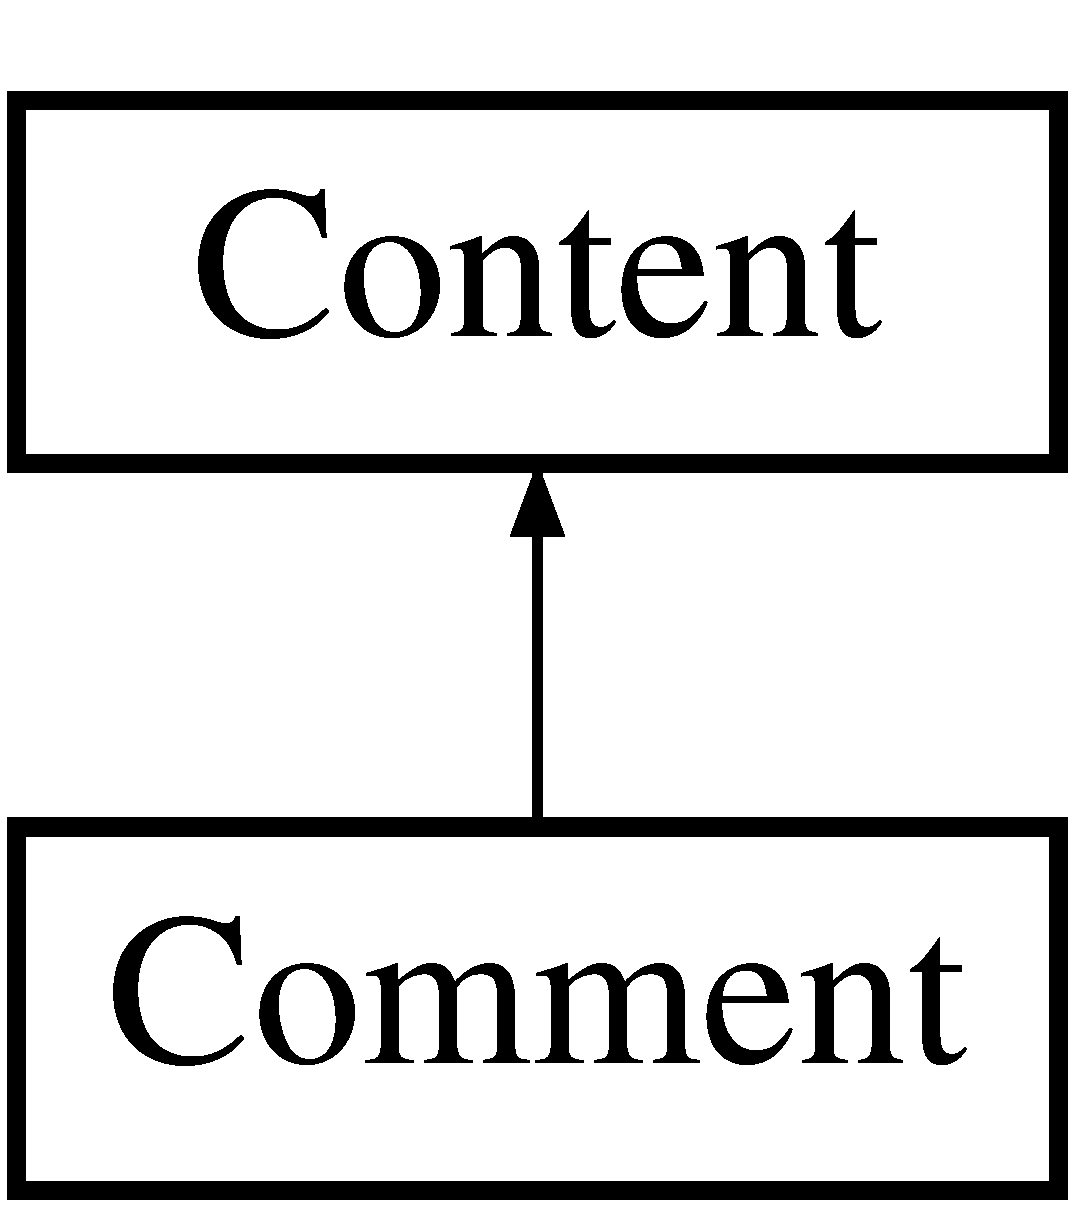
\includegraphics[height=2.000000cm]{class_comment}
\end{center}
\end{figure}
\subsection*{Public Member Functions}
\begin{DoxyCompactItemize}
\item 
\hyperlink{class_comment_a681be12288dbce6ceb0a6a6ae0c17c9c}{Comment} (\hyperlink{class_name}{Name}, \hyperlink{class_text}{Text})
\item 
\hyperlink{class_comment_aea2c5f6168b3bfdc1dbb7bb99ac44454}{$\sim$\+Comment} ()
\end{DoxyCompactItemize}
\subsection*{Additional Inherited Members}


\subsection{Constructor \& Destructor Documentation}
\mbox{\Hypertarget{class_comment_a681be12288dbce6ceb0a6a6ae0c17c9c}\label{class_comment_a681be12288dbce6ceb0a6a6ae0c17c9c}} 
\index{Comment@{Comment}!Comment@{Comment}}
\index{Comment@{Comment}!Comment@{Comment}}
\subsubsection{\texorpdfstring{Comment()}{Comment()}}
{\footnotesize\ttfamily Comment\+::\+Comment (\begin{DoxyParamCaption}\item[{\hyperlink{class_name}{Name}}]{author,  }\item[{\hyperlink{class_text}{Text}}]{comment\+\_\+content }\end{DoxyParamCaption})}

A public constructor. \mbox{\Hypertarget{class_comment_aea2c5f6168b3bfdc1dbb7bb99ac44454}\label{class_comment_aea2c5f6168b3bfdc1dbb7bb99ac44454}} 
\index{Comment@{Comment}!````~Comment@{$\sim$\+Comment}}
\index{````~Comment@{$\sim$\+Comment}!Comment@{Comment}}
\subsubsection{\texorpdfstring{$\sim$\+Comment()}{~Comment()}}
{\footnotesize\ttfamily Comment\+::$\sim$\+Comment (\begin{DoxyParamCaption}{ }\end{DoxyParamCaption})}

A public destructor. 

The documentation for this class was generated from the following files\+:\begin{DoxyCompactItemize}
\item 
\hyperlink{entities_8hpp}{entities.\+hpp}\item 
\hyperlink{entities_8cpp}{entities.\+cpp}\end{DoxyCompactItemize}

\hypertarget{class_content}{}\section{Content Class Reference}
\label{class_content}\index{Content@{Content}}


{\ttfamily \#include $<$entities.\+hpp$>$}

Inheritance diagram for Content\+:\begin{figure}[H]
\begin{center}
\leavevmode
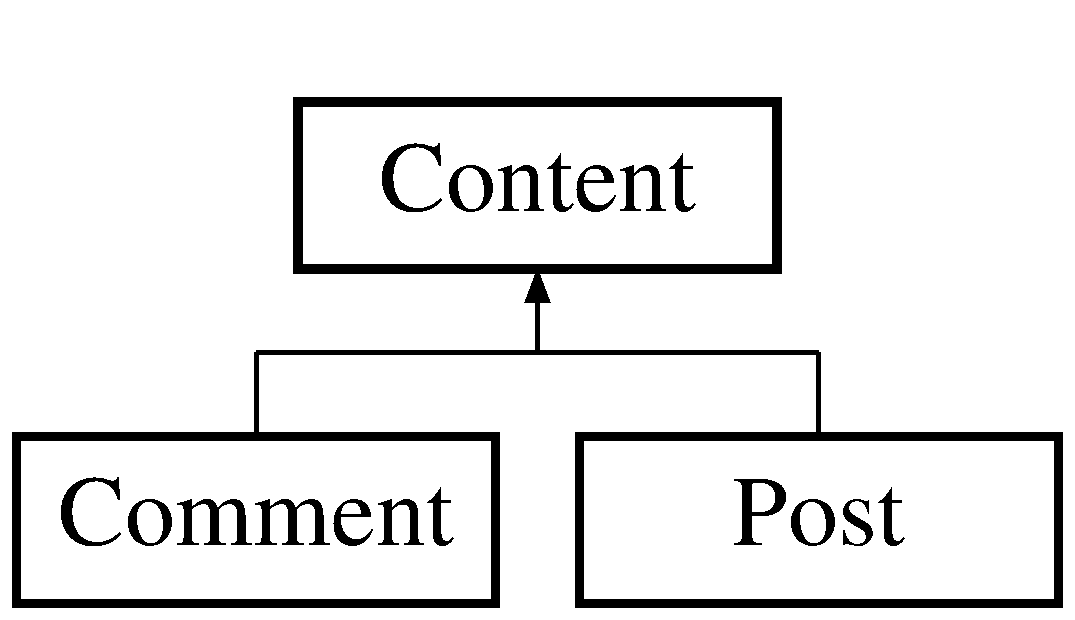
\includegraphics[height=2.000000cm]{class_content}
\end{center}
\end{figure}
\subsection*{Public Member Functions}
\begin{DoxyCompactItemize}
\item 
\hyperlink{class_content_af14b7b5ebc756686ecde73dc09b57c56}{Content} ()
\item 
\hyperlink{class_content_aa28dc7ed5866fb0c22dc13c2a1fdb495}{$\sim$\+Content} ()
\item 
\hyperlink{class_name}{Name} \hyperlink{class_content_a422f6d0fa9bbc258b4f2d2c32e825f73}{get\+\_\+author} ()
\item 
\hyperlink{class_text}{Text} \hyperlink{class_content_a855ce935e96e9c811ef84e0b20c38a59}{get\+\_\+content} ()
\item 
\hyperlink{class_avaliation}{Avaliation} \hyperlink{class_content_a82ec2dba39b5d5ac82ba3081e3a71548}{get\+\_\+avaliation} ()
\item 
void \hyperlink{class_content_a97a7150f5500238ca0de6f73073d8e71}{set} (\hyperlink{class_name}{Name}, \hyperlink{class_text}{Text})
\item 
void \hyperlink{class_content_a8dfaac49e63b4142dd68b30564838adf}{add\+\_\+avaliation} (\hyperlink{class_name}{Name}, \hyperlink{class_avaliation}{Avaliation})  throw (invalid\+\_\+argument)
\end{DoxyCompactItemize}
\subsection*{Protected Attributes}
\begin{DoxyCompactItemize}
\item 
\hyperlink{class_name}{Name} \hyperlink{class_content_a2b57299937210d9374f79624d44a4f33}{author}
\item 
\hyperlink{class_text}{Text} \hyperlink{class_content_a79390b6e1b8f81832a3b31bae4718148}{content}
\item 
map$<$ \hyperlink{class_name}{Name}, bool $>$ \hyperlink{class_content_a5203ffeb9ce422d8e8ea1d58dd44312a}{has\+\_\+avaliated}
\item 
vector$<$ \hyperlink{class_avaliation}{Avaliation} $>$ \hyperlink{class_content_aaa48d760bd18b48d17204c1532993c3b}{avaliations}
\end{DoxyCompactItemize}


\subsection{Constructor \& Destructor Documentation}
\mbox{\Hypertarget{class_content_af14b7b5ebc756686ecde73dc09b57c56}\label{class_content_af14b7b5ebc756686ecde73dc09b57c56}} 
\index{Content@{Content}!Content@{Content}}
\index{Content@{Content}!Content@{Content}}
\subsubsection{\texorpdfstring{Content()}{Content()}}
{\footnotesize\ttfamily Content\+::\+Content (\begin{DoxyParamCaption}{ }\end{DoxyParamCaption})}

A public constructor. \mbox{\Hypertarget{class_content_aa28dc7ed5866fb0c22dc13c2a1fdb495}\label{class_content_aa28dc7ed5866fb0c22dc13c2a1fdb495}} 
\index{Content@{Content}!````~Content@{$\sim$\+Content}}
\index{````~Content@{$\sim$\+Content}!Content@{Content}}
\subsubsection{\texorpdfstring{$\sim$\+Content()}{~Content()}}
{\footnotesize\ttfamily Content\+::$\sim$\+Content (\begin{DoxyParamCaption}{ }\end{DoxyParamCaption})}

A public destructor. 

\subsection{Member Function Documentation}
\mbox{\Hypertarget{class_content_a8dfaac49e63b4142dd68b30564838adf}\label{class_content_a8dfaac49e63b4142dd68b30564838adf}} 
\index{Content@{Content}!add\+\_\+avaliation@{add\+\_\+avaliation}}
\index{add\+\_\+avaliation@{add\+\_\+avaliation}!Content@{Content}}
\subsubsection{\texorpdfstring{add\+\_\+avaliation()}{add\_avaliation()}}
{\footnotesize\ttfamily void Content\+::add\+\_\+avaliation (\begin{DoxyParamCaption}\item[{\hyperlink{class_name}{Name}}]{name,  }\item[{\hyperlink{class_avaliation}{Avaliation}}]{avaliation }\end{DoxyParamCaption}) throw  invalid\+\_\+argument) }

A public method. Add an avaliation, making sure that no user do more than one avaliation. It receives a the name of the current user and the avaliation. \mbox{\Hypertarget{class_content_a422f6d0fa9bbc258b4f2d2c32e825f73}\label{class_content_a422f6d0fa9bbc258b4f2d2c32e825f73}} 
\index{Content@{Content}!get\+\_\+author@{get\+\_\+author}}
\index{get\+\_\+author@{get\+\_\+author}!Content@{Content}}
\subsubsection{\texorpdfstring{get\+\_\+author()}{get\_author()}}
{\footnotesize\ttfamily \hyperlink{class_name}{Name} Content\+::get\+\_\+author (\begin{DoxyParamCaption}{ }\end{DoxyParamCaption})}

A public method \begin{DoxyReturn}{Returns}
Value of the author of the content. 
\end{DoxyReturn}
\mbox{\Hypertarget{class_content_a82ec2dba39b5d5ac82ba3081e3a71548}\label{class_content_a82ec2dba39b5d5ac82ba3081e3a71548}} 
\index{Content@{Content}!get\+\_\+avaliation@{get\+\_\+avaliation}}
\index{get\+\_\+avaliation@{get\+\_\+avaliation}!Content@{Content}}
\subsubsection{\texorpdfstring{get\+\_\+avaliation()}{get\_avaliation()}}
{\footnotesize\ttfamily \hyperlink{class_avaliation}{Avaliation} Content\+::get\+\_\+avaliation (\begin{DoxyParamCaption}{ }\end{DoxyParamCaption})}

A public method \begin{DoxyReturn}{Returns}
The arithmetic mean of all avaliations given the to content in question. 
\end{DoxyReturn}
\mbox{\Hypertarget{class_content_a855ce935e96e9c811ef84e0b20c38a59}\label{class_content_a855ce935e96e9c811ef84e0b20c38a59}} 
\index{Content@{Content}!get\+\_\+content@{get\+\_\+content}}
\index{get\+\_\+content@{get\+\_\+content}!Content@{Content}}
\subsubsection{\texorpdfstring{get\+\_\+content()}{get\_content()}}
{\footnotesize\ttfamily \hyperlink{class_text}{Text} Content\+::get\+\_\+content (\begin{DoxyParamCaption}{ }\end{DoxyParamCaption})}

A public method \begin{DoxyReturn}{Returns}
Value of the content. 
\end{DoxyReturn}
\mbox{\Hypertarget{class_content_a97a7150f5500238ca0de6f73073d8e71}\label{class_content_a97a7150f5500238ca0de6f73073d8e71}} 
\index{Content@{Content}!set@{set}}
\index{set@{set}!Content@{Content}}
\subsubsection{\texorpdfstring{set()}{set()}}
{\footnotesize\ttfamily void Content\+::set (\begin{DoxyParamCaption}\item[{\hyperlink{class_name}{Name}}]{author,  }\item[{\hyperlink{class_text}{Text}}]{content }\end{DoxyParamCaption})}

A public method It receives the name of the author of the content and the content and valid them. 

\subsection{Member Data Documentation}
\mbox{\Hypertarget{class_content_a2b57299937210d9374f79624d44a4f33}\label{class_content_a2b57299937210d9374f79624d44a4f33}} 
\index{Content@{Content}!author@{author}}
\index{author@{author}!Content@{Content}}
\subsubsection{\texorpdfstring{author}{author}}
{\footnotesize\ttfamily \hyperlink{class_name}{Name} Content\+::author\hspace{0.3cm}{\ttfamily [protected]}}

A protected variable of class \hyperlink{class_name}{Name}. Keeps the name of the author of the content. \mbox{\Hypertarget{class_content_aaa48d760bd18b48d17204c1532993c3b}\label{class_content_aaa48d760bd18b48d17204c1532993c3b}} 
\index{Content@{Content}!avaliations@{avaliations}}
\index{avaliations@{avaliations}!Content@{Content}}
\subsubsection{\texorpdfstring{avaliations}{avaliations}}
{\footnotesize\ttfamily vector$<$\hyperlink{class_avaliation}{Avaliation}$>$ Content\+::avaliations\hspace{0.3cm}{\ttfamily [protected]}}

A protected variable of class Vector. Keeps the avaliations. \mbox{\Hypertarget{class_content_a79390b6e1b8f81832a3b31bae4718148}\label{class_content_a79390b6e1b8f81832a3b31bae4718148}} 
\index{Content@{Content}!content@{content}}
\index{content@{content}!Content@{Content}}
\subsubsection{\texorpdfstring{content}{content}}
{\footnotesize\ttfamily \hyperlink{class_text}{Text} Content\+::content\hspace{0.3cm}{\ttfamily [protected]}}

A protected variable of class \hyperlink{class_text}{Text}. Keeps the content. \mbox{\Hypertarget{class_content_a5203ffeb9ce422d8e8ea1d58dd44312a}\label{class_content_a5203ffeb9ce422d8e8ea1d58dd44312a}} 
\index{Content@{Content}!has\+\_\+avaliated@{has\+\_\+avaliated}}
\index{has\+\_\+avaliated@{has\+\_\+avaliated}!Content@{Content}}
\subsubsection{\texorpdfstring{has\+\_\+avaliated}{has\_avaliated}}
{\footnotesize\ttfamily map$<$\hyperlink{class_name}{Name}, bool$>$ Content\+::has\+\_\+avaliated\hspace{0.3cm}{\ttfamily [protected]}}

A protected variable of class Map. Keeps the name that everyone that has already avaliated. 

The documentation for this class was generated from the following files\+:\begin{DoxyCompactItemize}
\item 
\hyperlink{entities_8hpp}{entities.\+hpp}\item 
\hyperlink{entities_8cpp}{entities.\+cpp}\end{DoxyCompactItemize}

\hypertarget{class_domain}{}\section{Domain Class Reference}
\label{class_domain}\index{Domain@{Domain}}


{\ttfamily \#include $<$domains.\+hpp$>$}

Inheritance diagram for Domain\+:\begin{figure}[H]
\begin{center}
\leavevmode
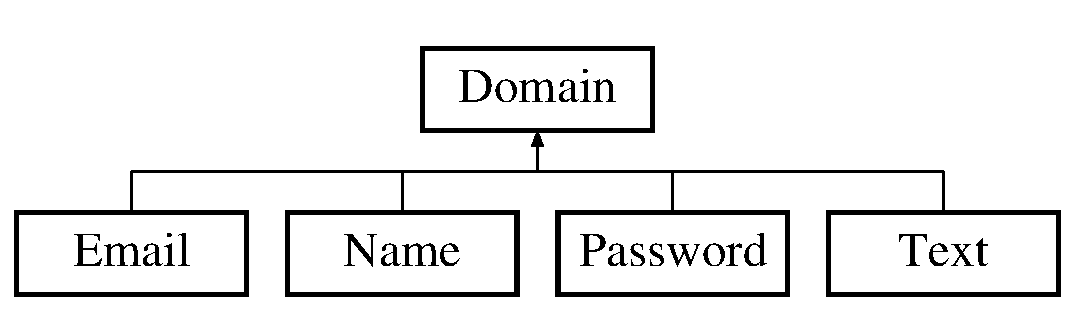
\includegraphics[height=2.000000cm]{class_domain}
\end{center}
\end{figure}
\subsection*{Public Member Functions}
\begin{DoxyCompactItemize}
\item 
\hyperlink{class_domain_a6adccae537e53d4fde2b70f875e6b8d0}{Domain} ()
\item 
\hyperlink{class_domain_a29cec9afb2e54c810ba1f3c1a49543a8}{$\sim$\+Domain} ()
\item 
string \hyperlink{class_domain_a265e5167062bf41ec78e4245af288c33}{get} ()
\item 
bool \hyperlink{class_domain_ae36e552d1a3bde70b7f448de345a3c9d}{empty} ()
\item 
void \hyperlink{class_domain_a629126b8c9a6a749d30745bde230c4ee}{set} (string)
\item 
bool \hyperlink{class_domain_a2791934de616d1bddcd93206b132c323}{operator!=} (const \hyperlink{class_domain}{Domain} \&other) const
\item 
bool \hyperlink{class_domain_acd0015ed9d54a761f7fca726fa53b541}{operator==} (const \hyperlink{class_domain}{Domain} \&other) const
\item 
bool \hyperlink{class_domain_ac165cf81dfabb07fbfdf0559525fc773}{operator$<$} (const \hyperlink{class_domain}{Domain} \&other) const
\end{DoxyCompactItemize}
\subsection*{Protected Member Functions}
\begin{DoxyCompactItemize}
\item 
virtual void \hyperlink{class_domain_a6a4590a4c94ae7be6f4f0da9703fb6d6}{valid} (string)=0  throw (invalid\+\_\+argument)
\end{DoxyCompactItemize}
\subsection*{Protected Attributes}
\begin{DoxyCompactItemize}
\item 
string \hyperlink{class_domain_a9d15a9f2c19c5863fe863a7d2f53a7cc}{value}
\end{DoxyCompactItemize}


\subsection{Detailed Description}
An Abstract Class \hyperlink{class_domain}{Domain}. Keeps a string for all classes that inherit this class and implement the methods get and set (respectively, see and modify the value keeped). Also declares a virtual method \char`\"{}valid\char`\"{} for each class implement. 

\subsection{Constructor \& Destructor Documentation}
\mbox{\Hypertarget{class_domain_a6adccae537e53d4fde2b70f875e6b8d0}\label{class_domain_a6adccae537e53d4fde2b70f875e6b8d0}} 
\index{Domain@{Domain}!Domain@{Domain}}
\index{Domain@{Domain}!Domain@{Domain}}
\subsubsection{\texorpdfstring{Domain()}{Domain()}}
{\footnotesize\ttfamily Domain\+::\+Domain (\begin{DoxyParamCaption}{ }\end{DoxyParamCaption})}

A public constructor. \mbox{\Hypertarget{class_domain_a29cec9afb2e54c810ba1f3c1a49543a8}\label{class_domain_a29cec9afb2e54c810ba1f3c1a49543a8}} 
\index{Domain@{Domain}!````~Domain@{$\sim$\+Domain}}
\index{````~Domain@{$\sim$\+Domain}!Domain@{Domain}}
\subsubsection{\texorpdfstring{$\sim$\+Domain()}{~Domain()}}
{\footnotesize\ttfamily Domain\+::$\sim$\+Domain (\begin{DoxyParamCaption}{ }\end{DoxyParamCaption})}

A public destructor. 

\subsection{Member Function Documentation}
\mbox{\Hypertarget{class_domain_ae36e552d1a3bde70b7f448de345a3c9d}\label{class_domain_ae36e552d1a3bde70b7f448de345a3c9d}} 
\index{Domain@{Domain}!empty@{empty}}
\index{empty@{empty}!Domain@{Domain}}
\subsubsection{\texorpdfstring{empty()}{empty()}}
{\footnotesize\ttfamily bool Domain\+::empty (\begin{DoxyParamCaption}{ }\end{DoxyParamCaption})}

A public method Warn if the string is empty. \mbox{\Hypertarget{class_domain_a265e5167062bf41ec78e4245af288c33}\label{class_domain_a265e5167062bf41ec78e4245af288c33}} 
\index{Domain@{Domain}!get@{get}}
\index{get@{get}!Domain@{Domain}}
\subsubsection{\texorpdfstring{get()}{get()}}
{\footnotesize\ttfamily string Domain\+::get (\begin{DoxyParamCaption}{ }\end{DoxyParamCaption})}

A public method \begin{DoxyReturn}{Returns}
Value of the keeped string. 
\end{DoxyReturn}
\mbox{\Hypertarget{class_domain_a2791934de616d1bddcd93206b132c323}\label{class_domain_a2791934de616d1bddcd93206b132c323}} 
\index{Domain@{Domain}!operator"!=@{operator"!=}}
\index{operator"!=@{operator"!=}!Domain@{Domain}}
\subsubsection{\texorpdfstring{operator"!=()}{operator!=()}}
{\footnotesize\ttfamily bool Domain\+::operator!= (\begin{DoxyParamCaption}\item[{const \hyperlink{class_domain}{Domain} \&}]{other }\end{DoxyParamCaption}) const}

Make it possible to compare if one \hyperlink{class_domain}{Domain} object has different value than other. \mbox{\Hypertarget{class_domain_ac165cf81dfabb07fbfdf0559525fc773}\label{class_domain_ac165cf81dfabb07fbfdf0559525fc773}} 
\index{Domain@{Domain}!operator$<$@{operator$<$}}
\index{operator$<$@{operator$<$}!Domain@{Domain}}
\subsubsection{\texorpdfstring{operator$<$()}{operator<()}}
{\footnotesize\ttfamily bool Domain\+::operator$<$ (\begin{DoxyParamCaption}\item[{const \hyperlink{class_domain}{Domain} \&}]{other }\end{DoxyParamCaption}) const}

Make it possible to compare if one \hyperlink{class_domain}{Domain} object has better value than other. \mbox{\Hypertarget{class_domain_acd0015ed9d54a761f7fca726fa53b541}\label{class_domain_acd0015ed9d54a761f7fca726fa53b541}} 
\index{Domain@{Domain}!operator==@{operator==}}
\index{operator==@{operator==}!Domain@{Domain}}
\subsubsection{\texorpdfstring{operator==()}{operator==()}}
{\footnotesize\ttfamily bool Domain\+::operator== (\begin{DoxyParamCaption}\item[{const \hyperlink{class_domain}{Domain} \&}]{other }\end{DoxyParamCaption}) const}

Make it possible to compare if one \hyperlink{class_domain}{Domain} object has igual value than other. \mbox{\Hypertarget{class_domain_a629126b8c9a6a749d30745bde230c4ee}\label{class_domain_a629126b8c9a6a749d30745bde230c4ee}} 
\index{Domain@{Domain}!set@{set}}
\index{set@{set}!Domain@{Domain}}
\subsubsection{\texorpdfstring{set()}{set()}}
{\footnotesize\ttfamily void Domain\+::set (\begin{DoxyParamCaption}\item[{string}]{value }\end{DoxyParamCaption})}

A public method Modify the value of the keeped string. \mbox{\Hypertarget{class_domain_a6a4590a4c94ae7be6f4f0da9703fb6d6}\label{class_domain_a6a4590a4c94ae7be6f4f0da9703fb6d6}} 
\index{Domain@{Domain}!valid@{valid}}
\index{valid@{valid}!Domain@{Domain}}
\subsubsection{\texorpdfstring{valid()}{valid()}}
{\footnotesize\ttfamily virtual void Domain\+::valid (\begin{DoxyParamCaption}\item[{string}]{ }\end{DoxyParamCaption}) throw  invalid\+\_\+argument) \hspace{0.3cm}{\ttfamily [protected]}, {\ttfamily [pure virtual]}}

A virtual method. For all classes that inherit this implement their own validation. Utilized in method set. 

\subsection{Member Data Documentation}
\mbox{\Hypertarget{class_domain_a9d15a9f2c19c5863fe863a7d2f53a7cc}\label{class_domain_a9d15a9f2c19c5863fe863a7d2f53a7cc}} 
\index{Domain@{Domain}!value@{value}}
\index{value@{value}!Domain@{Domain}}
\subsubsection{\texorpdfstring{value}{value}}
{\footnotesize\ttfamily string Domain\+::value\hspace{0.3cm}{\ttfamily [protected]}}

A protected string. Keep a value for all classes that inherit this one. 

The documentation for this class was generated from the following files\+:\begin{DoxyCompactItemize}
\item 
\hyperlink{domains_8hpp}{domains.\+hpp}\item 
\hyperlink{domains_8cpp}{domains.\+cpp}\end{DoxyCompactItemize}

\hypertarget{class_email}{}\section{Email Class Reference}
\label{class_email}\index{Email@{Email}}


{\ttfamily \#include $<$domains.\+hpp$>$}

Inheritance diagram for Email\+:\begin{figure}[H]
\begin{center}
\leavevmode
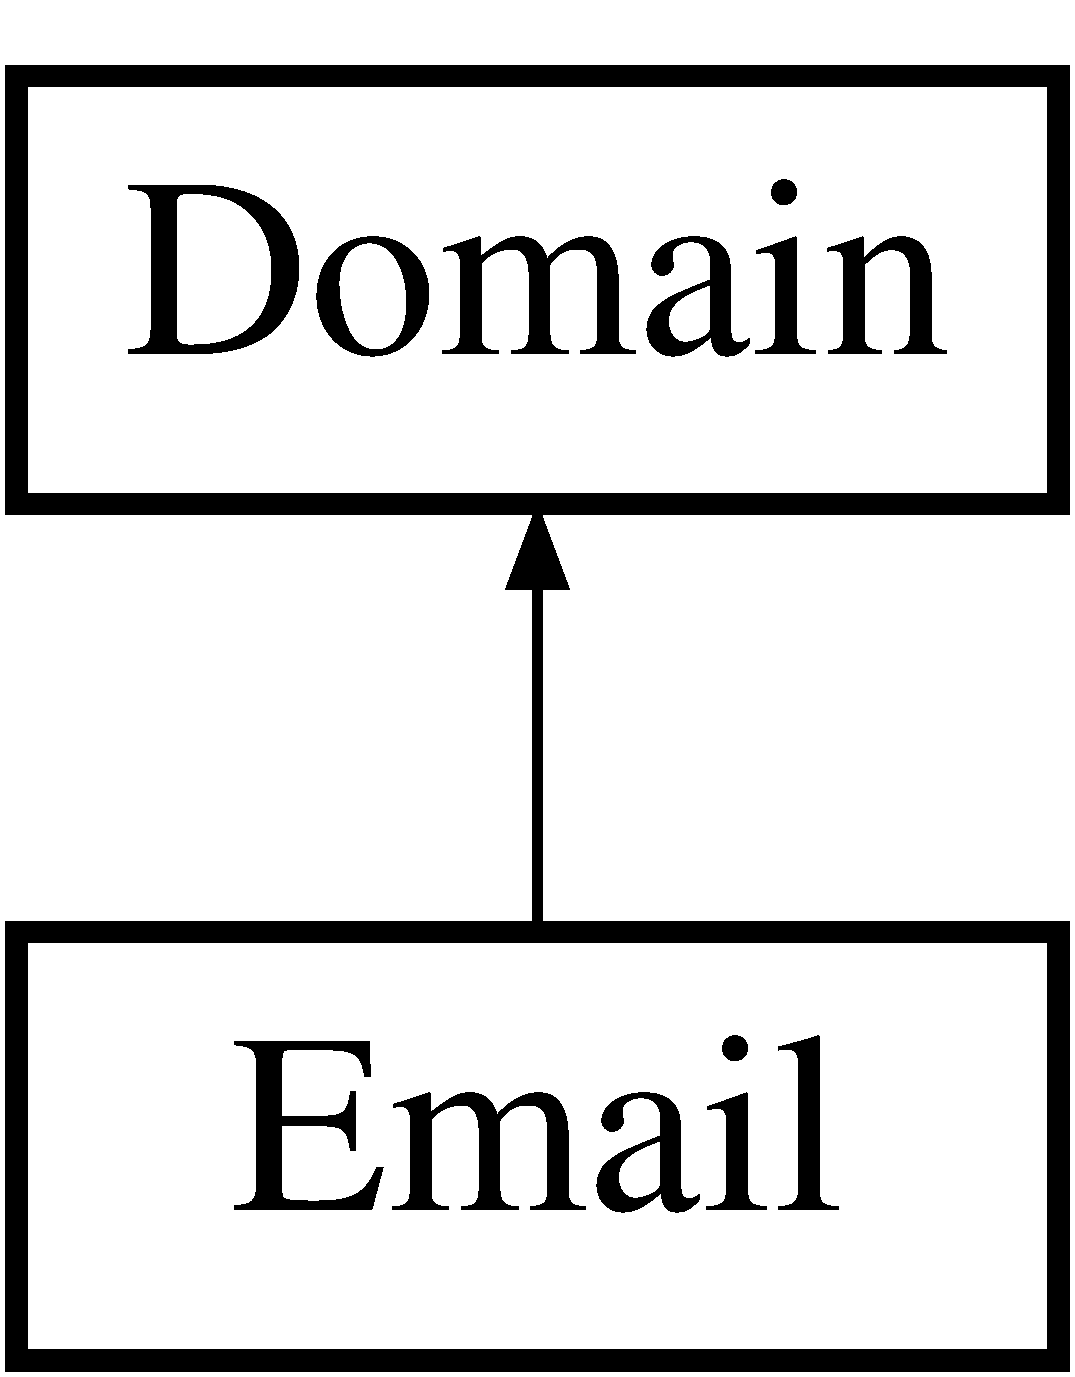
\includegraphics[height=2.000000cm]{class_email}
\end{center}
\end{figure}
\subsection*{Public Member Functions}
\begin{DoxyCompactItemize}
\item 
\hyperlink{class_email_a2cfcfea1e55511208e7858c33f48ad9d}{Email} ()
\item 
\hyperlink{class_email_a3e56bac4e1d6170fb5ba3ece6efb89a3}{$\sim$\+Email} ()
\end{DoxyCompactItemize}
\subsection*{Additional Inherited Members}


\subsection{Detailed Description}
A class \hyperlink{class_email}{Email}. Inherit of class \hyperlink{class_domain}{Domain}. Valid email. Verify if the email follow the pattern l.l (being l any string with only alphabetic caracters). 

\subsection{Constructor \& Destructor Documentation}
\mbox{\Hypertarget{class_email_a2cfcfea1e55511208e7858c33f48ad9d}\label{class_email_a2cfcfea1e55511208e7858c33f48ad9d}} 
\index{Email@{Email}!Email@{Email}}
\index{Email@{Email}!Email@{Email}}
\subsubsection{\texorpdfstring{Email()}{Email()}}
{\footnotesize\ttfamily Email\+::\+Email (\begin{DoxyParamCaption}{ }\end{DoxyParamCaption})}

A public constructor. \mbox{\Hypertarget{class_email_a3e56bac4e1d6170fb5ba3ece6efb89a3}\label{class_email_a3e56bac4e1d6170fb5ba3ece6efb89a3}} 
\index{Email@{Email}!````~Email@{$\sim$\+Email}}
\index{````~Email@{$\sim$\+Email}!Email@{Email}}
\subsubsection{\texorpdfstring{$\sim$\+Email()}{~Email()}}
{\footnotesize\ttfamily Email\+::$\sim$\+Email (\begin{DoxyParamCaption}{ }\end{DoxyParamCaption})}

A public destructor. 

The documentation for this class was generated from the following files\+:\begin{DoxyCompactItemize}
\item 
\hyperlink{domains_8hpp}{domains.\+hpp}\item 
\hyperlink{domains_8cpp}{domains.\+cpp}\end{DoxyCompactItemize}

\hypertarget{class_name}{}\section{Name Class Reference}
\label{class_name}\index{Name@{Name}}


{\ttfamily \#include $<$domains.\+hpp$>$}

Inheritance diagram for Name\+:\begin{figure}[H]
\begin{center}
\leavevmode
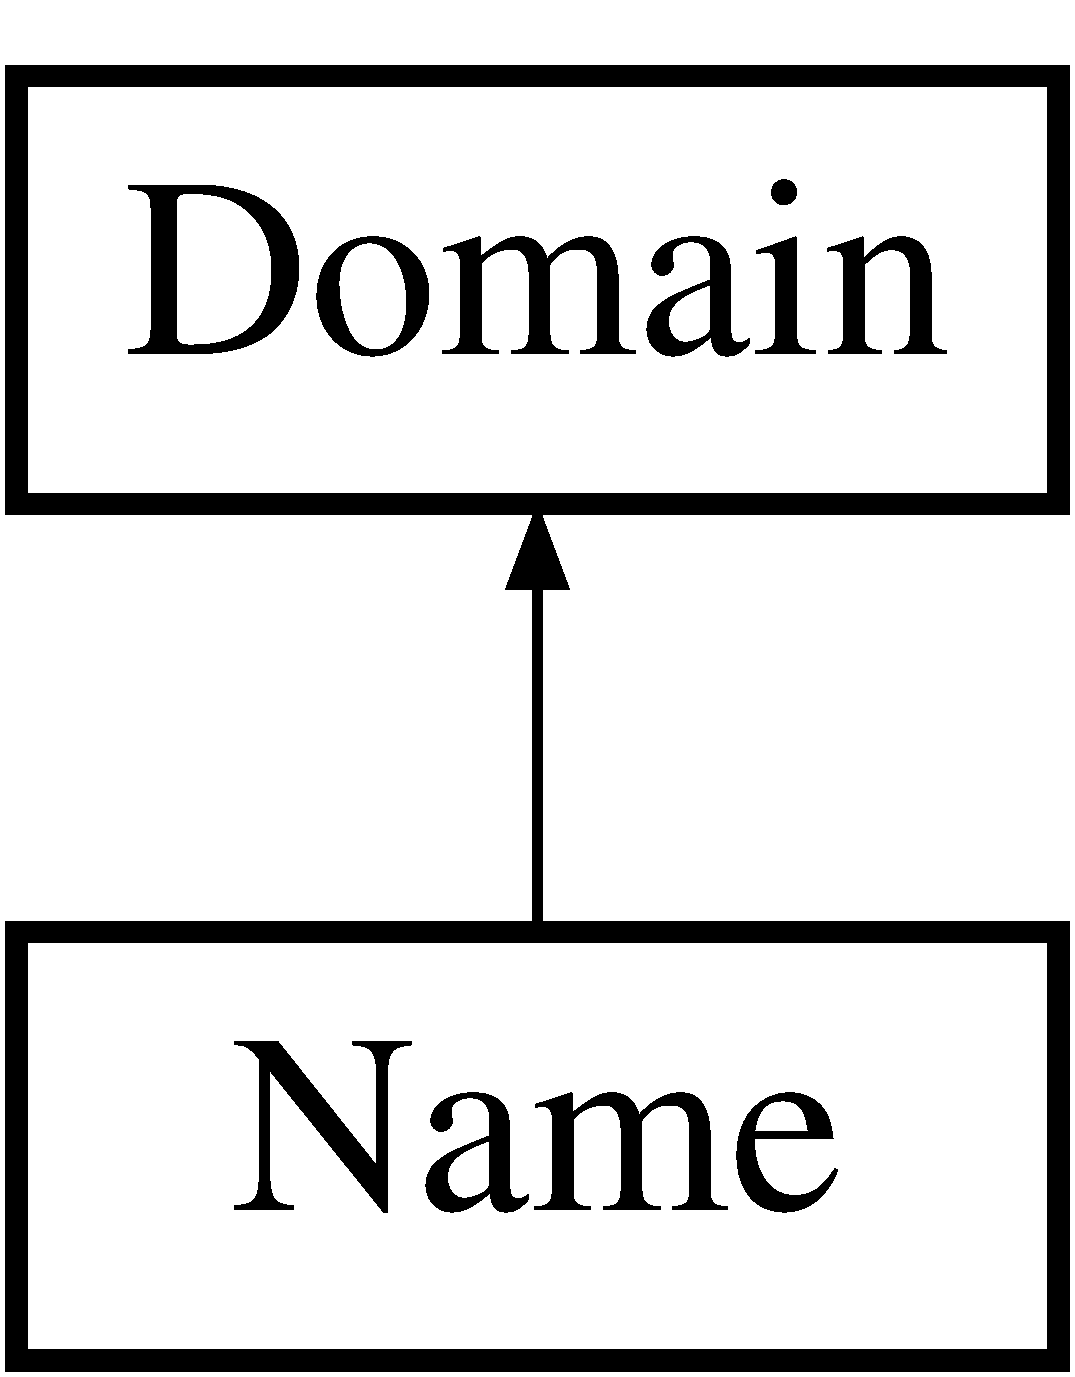
\includegraphics[height=2.000000cm]{class_name}
\end{center}
\end{figure}
\subsection*{Public Member Functions}
\begin{DoxyCompactItemize}
\item 
\hyperlink{class_name_a12a92d46d52b216ccaa86e3cb1539e58}{Name} ()
\item 
\hyperlink{class_name_ada9b23969d47506787d185c3fda43d77}{$\sim$\+Name} ()
\end{DoxyCompactItemize}
\subsection*{Additional Inherited Members}


\subsection{Detailed Description}
A class \hyperlink{class_name}{Name}. Inherit of class \hyperlink{class_domain}{Domain}. Valid name. Limit the size of the name. 

\subsection{Constructor \& Destructor Documentation}
\mbox{\Hypertarget{class_name_a12a92d46d52b216ccaa86e3cb1539e58}\label{class_name_a12a92d46d52b216ccaa86e3cb1539e58}} 
\index{Name@{Name}!Name@{Name}}
\index{Name@{Name}!Name@{Name}}
\subsubsection{\texorpdfstring{Name()}{Name()}}
{\footnotesize\ttfamily Name\+::\+Name (\begin{DoxyParamCaption}{ }\end{DoxyParamCaption})}

A public constructor. \mbox{\Hypertarget{class_name_ada9b23969d47506787d185c3fda43d77}\label{class_name_ada9b23969d47506787d185c3fda43d77}} 
\index{Name@{Name}!````~Name@{$\sim$\+Name}}
\index{````~Name@{$\sim$\+Name}!Name@{Name}}
\subsubsection{\texorpdfstring{$\sim$\+Name()}{~Name()}}
{\footnotesize\ttfamily Name\+::$\sim$\+Name (\begin{DoxyParamCaption}{ }\end{DoxyParamCaption})}

A public destructor. 

The documentation for this class was generated from the following files\+:\begin{DoxyCompactItemize}
\item 
\hyperlink{domains_8hpp}{domains.\+hpp}\item 
\hyperlink{domains_8cpp}{domains.\+cpp}\end{DoxyCompactItemize}

\hypertarget{class_password}{}\section{Password Class Reference}
\label{class_password}\index{Password@{Password}}


{\ttfamily \#include $<$domains.\+hpp$>$}

Inheritance diagram for Password\+:\begin{figure}[H]
\begin{center}
\leavevmode
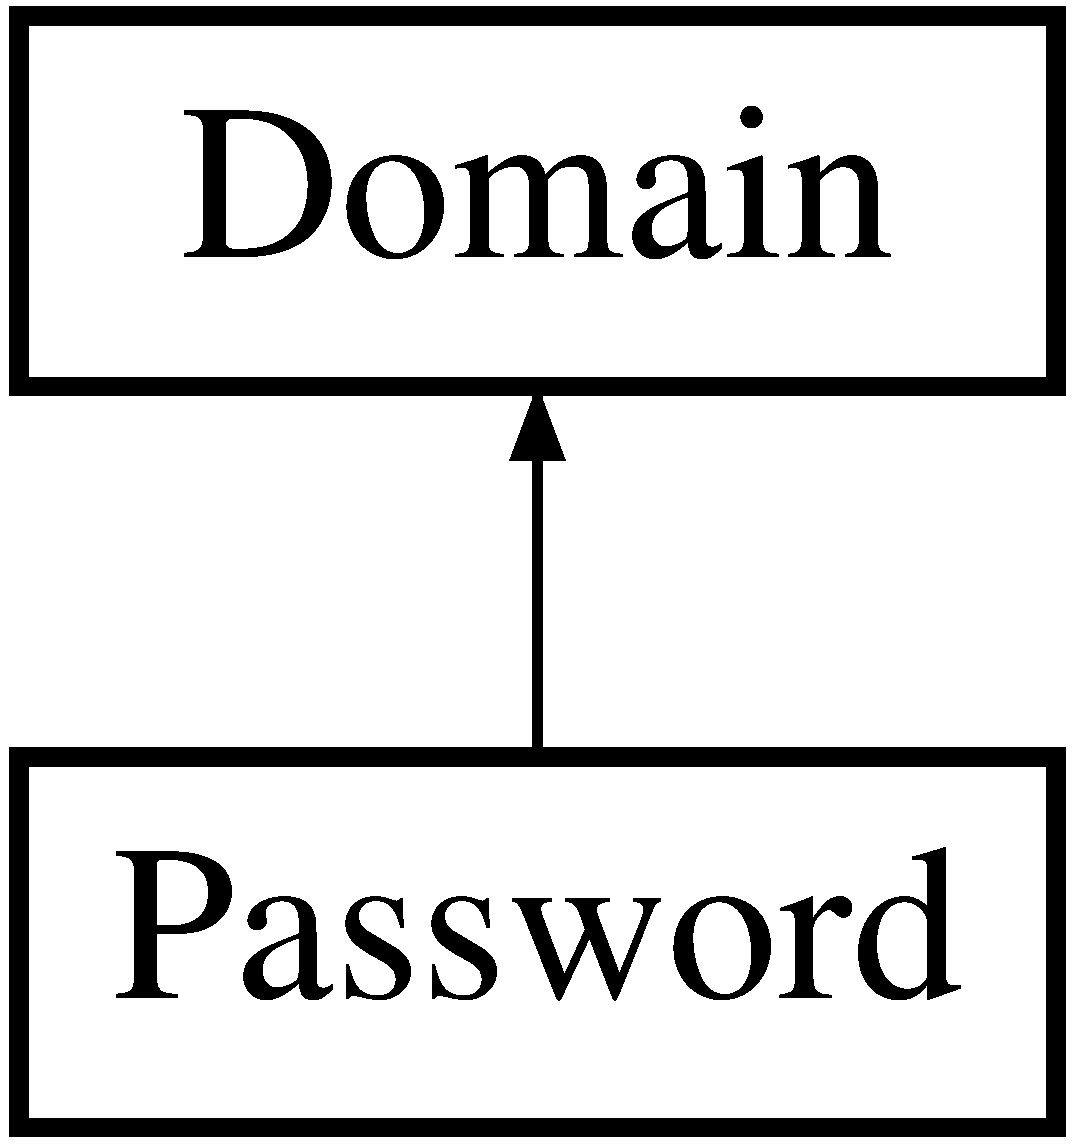
\includegraphics[height=2.000000cm]{class_password}
\end{center}
\end{figure}
\subsection*{Public Member Functions}
\begin{DoxyCompactItemize}
\item 
\hyperlink{class_password_a9ed0401599b14d501a8f46779048cdf2}{Password} ()
\item 
\hyperlink{class_password_ae019a63cb7332cb1c4e41d8ab7b4a619}{$\sim$\+Password} ()
\end{DoxyCompactItemize}
\subsection*{Additional Inherited Members}


\subsection{Detailed Description}
A class \hyperlink{class_password}{Password}. Inherit of class \hyperlink{class_domain}{Domain}. Valid password. Define the size of the password and does not permit that more than 1 caracter repeats. 

\subsection{Constructor \& Destructor Documentation}
\mbox{\Hypertarget{class_password_a9ed0401599b14d501a8f46779048cdf2}\label{class_password_a9ed0401599b14d501a8f46779048cdf2}} 
\index{Password@{Password}!Password@{Password}}
\index{Password@{Password}!Password@{Password}}
\subsubsection{\texorpdfstring{Password()}{Password()}}
{\footnotesize\ttfamily Password\+::\+Password (\begin{DoxyParamCaption}{ }\end{DoxyParamCaption})}

A public constructor. \mbox{\Hypertarget{class_password_ae019a63cb7332cb1c4e41d8ab7b4a619}\label{class_password_ae019a63cb7332cb1c4e41d8ab7b4a619}} 
\index{Password@{Password}!````~Password@{$\sim$\+Password}}
\index{````~Password@{$\sim$\+Password}!Password@{Password}}
\subsubsection{\texorpdfstring{$\sim$\+Password()}{~Password()}}
{\footnotesize\ttfamily Password\+::$\sim$\+Password (\begin{DoxyParamCaption}{ }\end{DoxyParamCaption})}

A public destructor. 

The documentation for this class was generated from the following files\+:\begin{DoxyCompactItemize}
\item 
\hyperlink{domains_8hpp}{domains.\+hpp}\item 
\hyperlink{domains_8cpp}{domains.\+cpp}\end{DoxyCompactItemize}

\hypertarget{class_post}{}\section{Post Class Reference}
\label{class_post}\index{Post@{Post}}


{\ttfamily \#include $<$entities.\+hpp$>$}

Inheritance diagram for Post\+:\begin{figure}[H]
\begin{center}
\leavevmode
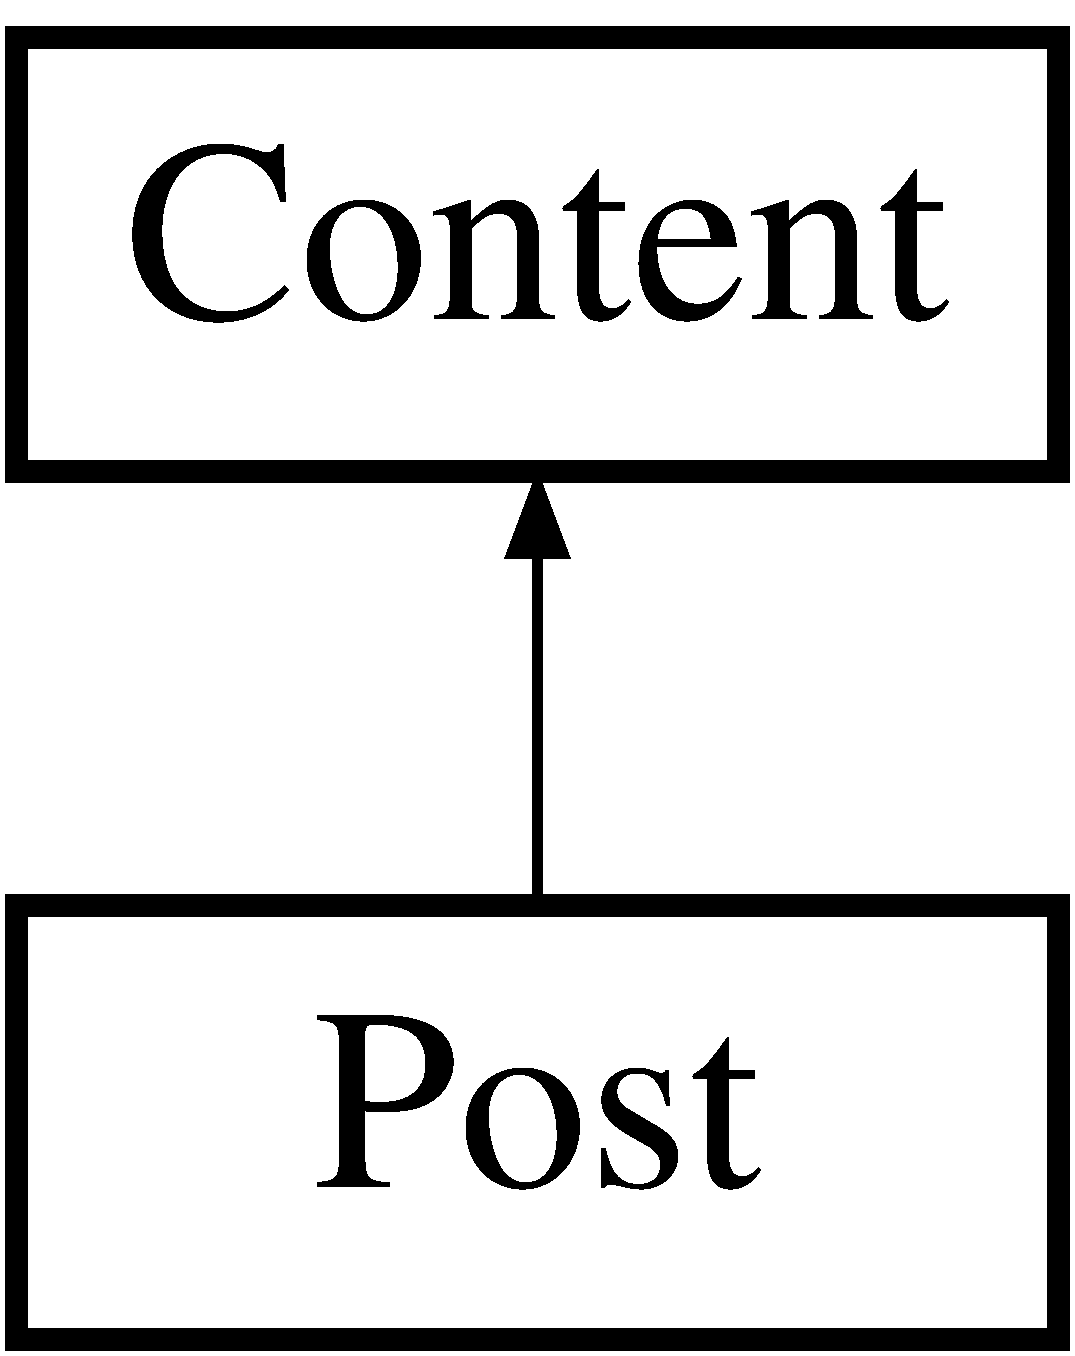
\includegraphics[height=2.000000cm]{class_post}
\end{center}
\end{figure}
\subsection*{Public Member Functions}
\begin{DoxyCompactItemize}
\item 
\hyperlink{class_post_ae548a55c0bfa09e805cd0a19b07db365}{Post} (\hyperlink{class_name}{Name}, \hyperlink{class_text}{Text})
\item 
\hyperlink{class_post_a6c1e585c0adb3220a154ba20d2144ae1}{$\sim$\+Post} ()
\item 
void \hyperlink{class_post_a8172722471012d2a6ede1a0b10c7f756}{allow\+\_\+comments} ()
\item 
void \hyperlink{class_post_ab2bf16185ad34d5cfca23785bc2a95e6}{disallow\+\_\+comments} ()
\item 
vector$<$ \hyperlink{class_comment}{Comment} $>$ \hyperlink{class_post_a026bd803b219f1cb373d3041c53261eb}{get\+\_\+comments} ()
\item 
void \hyperlink{class_post_a882ef59148fa556833a68fbdedce58da}{add\+\_\+comment} (\hyperlink{class_comment}{Comment})  throw (invalid\+\_\+argument)
\end{DoxyCompactItemize}
\subsection*{Additional Inherited Members}


\subsection{Constructor \& Destructor Documentation}
\mbox{\Hypertarget{class_post_ae548a55c0bfa09e805cd0a19b07db365}\label{class_post_ae548a55c0bfa09e805cd0a19b07db365}} 
\index{Post@{Post}!Post@{Post}}
\index{Post@{Post}!Post@{Post}}
\subsubsection{\texorpdfstring{Post()}{Post()}}
{\footnotesize\ttfamily Post\+::\+Post (\begin{DoxyParamCaption}\item[{\hyperlink{class_name}{Name}}]{author,  }\item[{\hyperlink{class_text}{Text}}]{post\+\_\+content }\end{DoxyParamCaption})}

A public constructor. \mbox{\Hypertarget{class_post_a6c1e585c0adb3220a154ba20d2144ae1}\label{class_post_a6c1e585c0adb3220a154ba20d2144ae1}} 
\index{Post@{Post}!````~Post@{$\sim$\+Post}}
\index{````~Post@{$\sim$\+Post}!Post@{Post}}
\subsubsection{\texorpdfstring{$\sim$\+Post()}{~Post()}}
{\footnotesize\ttfamily Post\+::$\sim$\+Post (\begin{DoxyParamCaption}{ }\end{DoxyParamCaption})}

A public destructor. 

\subsection{Member Function Documentation}
\mbox{\Hypertarget{class_post_a882ef59148fa556833a68fbdedce58da}\label{class_post_a882ef59148fa556833a68fbdedce58da}} 
\index{Post@{Post}!add\+\_\+comment@{add\+\_\+comment}}
\index{add\+\_\+comment@{add\+\_\+comment}!Post@{Post}}
\subsubsection{\texorpdfstring{add\+\_\+comment()}{add\_comment()}}
{\footnotesize\ttfamily void Post\+::add\+\_\+comment (\begin{DoxyParamCaption}\item[{\hyperlink{class_comment}{Comment}}]{comment }\end{DoxyParamCaption}) throw  invalid\+\_\+argument) }

A public method Add a comment if possible (no user can comment more than 5 times and the post has to autorize comments). \mbox{\Hypertarget{class_post_a8172722471012d2a6ede1a0b10c7f756}\label{class_post_a8172722471012d2a6ede1a0b10c7f756}} 
\index{Post@{Post}!allow\+\_\+comments@{allow\+\_\+comments}}
\index{allow\+\_\+comments@{allow\+\_\+comments}!Post@{Post}}
\subsubsection{\texorpdfstring{allow\+\_\+comments()}{allow\_comments()}}
{\footnotesize\ttfamily void Post\+::allow\+\_\+comments (\begin{DoxyParamCaption}{ }\end{DoxyParamCaption})}

A public method Allow comments to be made by other users. \mbox{\Hypertarget{class_post_ab2bf16185ad34d5cfca23785bc2a95e6}\label{class_post_ab2bf16185ad34d5cfca23785bc2a95e6}} 
\index{Post@{Post}!disallow\+\_\+comments@{disallow\+\_\+comments}}
\index{disallow\+\_\+comments@{disallow\+\_\+comments}!Post@{Post}}
\subsubsection{\texorpdfstring{disallow\+\_\+comments()}{disallow\_comments()}}
{\footnotesize\ttfamily void Post\+::disallow\+\_\+comments (\begin{DoxyParamCaption}{ }\end{DoxyParamCaption})}

A public method Disallow comments. This excludes all current comments. \mbox{\Hypertarget{class_post_a026bd803b219f1cb373d3041c53261eb}\label{class_post_a026bd803b219f1cb373d3041c53261eb}} 
\index{Post@{Post}!get\+\_\+comments@{get\+\_\+comments}}
\index{get\+\_\+comments@{get\+\_\+comments}!Post@{Post}}
\subsubsection{\texorpdfstring{get\+\_\+comments()}{get\_comments()}}
{\footnotesize\ttfamily vector$<$ \hyperlink{class_comment}{Comment} $>$ Post\+::get\+\_\+comments (\begin{DoxyParamCaption}{ }\end{DoxyParamCaption})}

A public method \begin{DoxyReturn}{Returns}
all the comments. 
\end{DoxyReturn}


The documentation for this class was generated from the following files\+:\begin{DoxyCompactItemize}
\item 
\hyperlink{entities_8hpp}{entities.\+hpp}\item 
\hyperlink{entities_8cpp}{entities.\+cpp}\end{DoxyCompactItemize}

\hypertarget{class_test_avaliation}{}\section{Test\+Avaliation Class Reference}
\label{class_test_avaliation}\index{Test\+Avaliation@{Test\+Avaliation}}


{\ttfamily \#include $<$test\+\_\+domains.\+hpp$>$}

\subsection*{Public Member Functions}
\begin{DoxyCompactItemize}
\item 
void \hyperlink{class_test_avaliation_a8c6b9d3e1660e1cf24e335f90f22b2da}{verify} ()
\item 
\hyperlink{class_test_avaliation_adc24d227366745218f50c1add1b1af18}{Test\+Avaliation} ()
\item 
\hyperlink{class_test_avaliation_aafdef825a4b4cd68e91102abc249c751}{$\sim$\+Test\+Avaliation} ()
\end{DoxyCompactItemize}


\subsection{Constructor \& Destructor Documentation}
\mbox{\Hypertarget{class_test_avaliation_adc24d227366745218f50c1add1b1af18}\label{class_test_avaliation_adc24d227366745218f50c1add1b1af18}} 
\index{Test\+Avaliation@{Test\+Avaliation}!Test\+Avaliation@{Test\+Avaliation}}
\index{Test\+Avaliation@{Test\+Avaliation}!Test\+Avaliation@{Test\+Avaliation}}
\subsubsection{\texorpdfstring{Test\+Avaliation()}{TestAvaliation()}}
{\footnotesize\ttfamily Test\+Avaliation\+::\+Test\+Avaliation (\begin{DoxyParamCaption}{ }\end{DoxyParamCaption})}

A public constructor \mbox{\Hypertarget{class_test_avaliation_aafdef825a4b4cd68e91102abc249c751}\label{class_test_avaliation_aafdef825a4b4cd68e91102abc249c751}} 
\index{Test\+Avaliation@{Test\+Avaliation}!````~Test\+Avaliation@{$\sim$\+Test\+Avaliation}}
\index{````~Test\+Avaliation@{$\sim$\+Test\+Avaliation}!Test\+Avaliation@{Test\+Avaliation}}
\subsubsection{\texorpdfstring{$\sim$\+Test\+Avaliation()}{~TestAvaliation()}}
{\footnotesize\ttfamily Test\+Avaliation\+::$\sim$\+Test\+Avaliation (\begin{DoxyParamCaption}{ }\end{DoxyParamCaption})}

A public destructor 

\subsection{Member Function Documentation}
\mbox{\Hypertarget{class_test_avaliation_a8c6b9d3e1660e1cf24e335f90f22b2da}\label{class_test_avaliation_a8c6b9d3e1660e1cf24e335f90f22b2da}} 
\index{Test\+Avaliation@{Test\+Avaliation}!verify@{verify}}
\index{verify@{verify}!Test\+Avaliation@{Test\+Avaliation}}
\subsubsection{\texorpdfstring{verify()}{verify()}}
{\footnotesize\ttfamily void Test\+Avaliation\+::verify (\begin{DoxyParamCaption}{ }\end{DoxyParamCaption})}

A public method Call the test methods with the expected values 

The documentation for this class was generated from the following files\+:\begin{DoxyCompactItemize}
\item 
\hyperlink{test__domains_8hpp}{test\+\_\+domains.\+hpp}\item 
\hyperlink{test__domains_8cpp}{test\+\_\+domains.\+cpp}\end{DoxyCompactItemize}

\hypertarget{class_test_blog}{}\section{Test\+Blog Class Reference}
\label{class_test_blog}\index{Test\+Blog@{Test\+Blog}}


{\ttfamily \#include $<$test\+\_\+entities.\+hpp$>$}

\subsection*{Public Member Functions}
\begin{DoxyCompactItemize}
\item 
\hyperlink{class_test_blog_a63740a7abdb9db8a0b43ec8e9916cd84}{Test\+Blog} ()
\item 
\hyperlink{class_test_blog_ad8e8737a111da9f41f75c6882d645ca4}{$\sim$\+Test\+Blog} ()
\item 
void \hyperlink{class_test_blog_a927d67cdfb5807554fef14270cb927dd}{verify} ()
\end{DoxyCompactItemize}


\subsection{Constructor \& Destructor Documentation}
\mbox{\Hypertarget{class_test_blog_a63740a7abdb9db8a0b43ec8e9916cd84}\label{class_test_blog_a63740a7abdb9db8a0b43ec8e9916cd84}} 
\index{Test\+Blog@{Test\+Blog}!Test\+Blog@{Test\+Blog}}
\index{Test\+Blog@{Test\+Blog}!Test\+Blog@{Test\+Blog}}
\subsubsection{\texorpdfstring{Test\+Blog()}{TestBlog()}}
{\footnotesize\ttfamily Test\+Blog\+::\+Test\+Blog (\begin{DoxyParamCaption}{ }\end{DoxyParamCaption})}

A public constructor \mbox{\Hypertarget{class_test_blog_ad8e8737a111da9f41f75c6882d645ca4}\label{class_test_blog_ad8e8737a111da9f41f75c6882d645ca4}} 
\index{Test\+Blog@{Test\+Blog}!````~Test\+Blog@{$\sim$\+Test\+Blog}}
\index{````~Test\+Blog@{$\sim$\+Test\+Blog}!Test\+Blog@{Test\+Blog}}
\subsubsection{\texorpdfstring{$\sim$\+Test\+Blog()}{~TestBlog()}}
{\footnotesize\ttfamily Test\+Blog\+::$\sim$\+Test\+Blog (\begin{DoxyParamCaption}{ }\end{DoxyParamCaption})}

A public destructor 

\subsection{Member Function Documentation}
\mbox{\Hypertarget{class_test_blog_a927d67cdfb5807554fef14270cb927dd}\label{class_test_blog_a927d67cdfb5807554fef14270cb927dd}} 
\index{Test\+Blog@{Test\+Blog}!verify@{verify}}
\index{verify@{verify}!Test\+Blog@{Test\+Blog}}
\subsubsection{\texorpdfstring{verify()}{verify()}}
{\footnotesize\ttfamily void Test\+Blog\+::verify (\begin{DoxyParamCaption}{ }\end{DoxyParamCaption})}

A public method Call the test methods with the expected values 

The documentation for this class was generated from the following files\+:\begin{DoxyCompactItemize}
\item 
\hyperlink{test__entities_8hpp}{test\+\_\+entities.\+hpp}\item 
\hyperlink{test__entities_8cpp}{test\+\_\+entities.\+cpp}\end{DoxyCompactItemize}

\hypertarget{class_test_comment}{}\section{Test\+Comment Class Reference}
\label{class_test_comment}\index{Test\+Comment@{Test\+Comment}}


{\ttfamily \#include $<$test\+\_\+entities.\+hpp$>$}

\subsection*{Public Member Functions}
\begin{DoxyCompactItemize}
\item 
\hyperlink{class_test_comment_aa12b638387e03b63fcac02ca5b064b74}{Test\+Comment} ()
\item 
\hyperlink{class_test_comment_af26a10325ebf5c69372b77243dc1bf18}{$\sim$\+Test\+Comment} ()
\item 
void \hyperlink{class_test_comment_a35b7553c77a3922bf0739b8d39073948}{verify} ()
\end{DoxyCompactItemize}


\subsection{Constructor \& Destructor Documentation}
\mbox{\Hypertarget{class_test_comment_aa12b638387e03b63fcac02ca5b064b74}\label{class_test_comment_aa12b638387e03b63fcac02ca5b064b74}} 
\index{Test\+Comment@{Test\+Comment}!Test\+Comment@{Test\+Comment}}
\index{Test\+Comment@{Test\+Comment}!Test\+Comment@{Test\+Comment}}
\subsubsection{\texorpdfstring{Test\+Comment()}{TestComment()}}
{\footnotesize\ttfamily Test\+Comment\+::\+Test\+Comment (\begin{DoxyParamCaption}{ }\end{DoxyParamCaption})}

A public constructor \mbox{\Hypertarget{class_test_comment_af26a10325ebf5c69372b77243dc1bf18}\label{class_test_comment_af26a10325ebf5c69372b77243dc1bf18}} 
\index{Test\+Comment@{Test\+Comment}!````~Test\+Comment@{$\sim$\+Test\+Comment}}
\index{````~Test\+Comment@{$\sim$\+Test\+Comment}!Test\+Comment@{Test\+Comment}}
\subsubsection{\texorpdfstring{$\sim$\+Test\+Comment()}{~TestComment()}}
{\footnotesize\ttfamily Test\+Comment\+::$\sim$\+Test\+Comment (\begin{DoxyParamCaption}{ }\end{DoxyParamCaption})}

A public destructor 

\subsection{Member Function Documentation}
\mbox{\Hypertarget{class_test_comment_a35b7553c77a3922bf0739b8d39073948}\label{class_test_comment_a35b7553c77a3922bf0739b8d39073948}} 
\index{Test\+Comment@{Test\+Comment}!verify@{verify}}
\index{verify@{verify}!Test\+Comment@{Test\+Comment}}
\subsubsection{\texorpdfstring{verify()}{verify()}}
{\footnotesize\ttfamily void Test\+Comment\+::verify (\begin{DoxyParamCaption}{ }\end{DoxyParamCaption})}

A public method Call the test methods with the expected values 

The documentation for this class was generated from the following files\+:\begin{DoxyCompactItemize}
\item 
\hyperlink{test__entities_8hpp}{test\+\_\+entities.\+hpp}\item 
\hyperlink{test__entities_8cpp}{test\+\_\+entities.\+cpp}\end{DoxyCompactItemize}

\hypertarget{class_test_domain}{}\section{Test\+Domain Class Reference}
\label{class_test_domain}\index{Test\+Domain@{Test\+Domain}}


{\ttfamily \#include $<$test\+\_\+domains.\+hpp$>$}

Inheritance diagram for Test\+Domain\+:\begin{figure}[H]
\begin{center}
\leavevmode
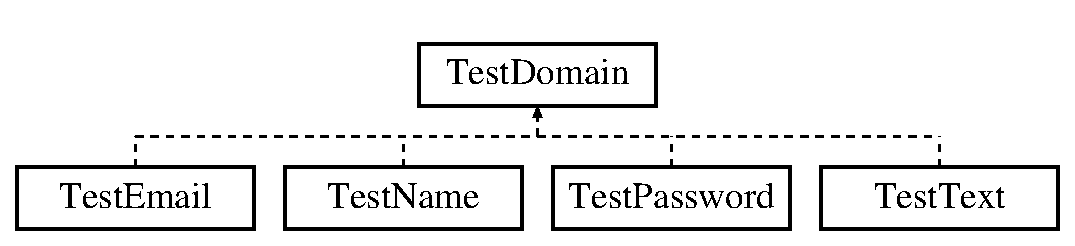
\includegraphics[height=2.000000cm]{class_test_domain}
\end{center}
\end{figure}
\subsection*{Public Member Functions}
\begin{DoxyCompactItemize}
\item 
\hyperlink{class_test_domain_aca311894bf6af9feb53c83a3659f208b}{Test\+Domain} ()
\item 
\hyperlink{class_test_domain_ab5be880050c36e6dcc470a452b4b9f69}{$\sim$\+Test\+Domain} ()
\end{DoxyCompactItemize}
\subsection*{Protected Member Functions}
\begin{DoxyCompactItemize}
\item 
void \hyperlink{class_test_domain_a9945e79f1f6d965e6b58f149b2c8cf84}{success\+\_\+scenario} (string, \hyperlink{class_domain}{Domain} \&)  throw (invalid\+\_\+argument)
\item 
void \hyperlink{class_test_domain_a026682e48bdb2ffdf6b3d353c7f055fe}{failure\+\_\+scenario} (string, \hyperlink{class_domain}{Domain} \&)  throw (invalid\+\_\+argument)
\end{DoxyCompactItemize}


\subsection{Constructor \& Destructor Documentation}
\mbox{\Hypertarget{class_test_domain_aca311894bf6af9feb53c83a3659f208b}\label{class_test_domain_aca311894bf6af9feb53c83a3659f208b}} 
\index{Test\+Domain@{Test\+Domain}!Test\+Domain@{Test\+Domain}}
\index{Test\+Domain@{Test\+Domain}!Test\+Domain@{Test\+Domain}}
\subsubsection{\texorpdfstring{Test\+Domain()}{TestDomain()}}
{\footnotesize\ttfamily Test\+Domain\+::\+Test\+Domain (\begin{DoxyParamCaption}{ }\end{DoxyParamCaption})}

A public constructor \mbox{\Hypertarget{class_test_domain_ab5be880050c36e6dcc470a452b4b9f69}\label{class_test_domain_ab5be880050c36e6dcc470a452b4b9f69}} 
\index{Test\+Domain@{Test\+Domain}!````~Test\+Domain@{$\sim$\+Test\+Domain}}
\index{````~Test\+Domain@{$\sim$\+Test\+Domain}!Test\+Domain@{Test\+Domain}}
\subsubsection{\texorpdfstring{$\sim$\+Test\+Domain()}{~TestDomain()}}
{\footnotesize\ttfamily Test\+Domain\+::$\sim$\+Test\+Domain (\begin{DoxyParamCaption}{ }\end{DoxyParamCaption})}

A public destructor 

\subsection{Member Function Documentation}
\mbox{\Hypertarget{class_test_domain_a026682e48bdb2ffdf6b3d353c7f055fe}\label{class_test_domain_a026682e48bdb2ffdf6b3d353c7f055fe}} 
\index{Test\+Domain@{Test\+Domain}!failure\+\_\+scenario@{failure\+\_\+scenario}}
\index{failure\+\_\+scenario@{failure\+\_\+scenario}!Test\+Domain@{Test\+Domain}}
\subsubsection{\texorpdfstring{failure\+\_\+scenario()}{failure\_scenario()}}
{\footnotesize\ttfamily void Test\+Domain\+::failure\+\_\+scenario (\begin{DoxyParamCaption}\item[{string}]{value,  }\item[{\hyperlink{class_domain}{Domain} \&}]{test\+Auxiliar }\end{DoxyParamCaption}) throw  invalid\+\_\+argument) \hspace{0.3cm}{\ttfamily [protected]}}

A protected method Test the methods of the receivied class and throw exception if something wrong is not detected \mbox{\Hypertarget{class_test_domain_a9945e79f1f6d965e6b58f149b2c8cf84}\label{class_test_domain_a9945e79f1f6d965e6b58f149b2c8cf84}} 
\index{Test\+Domain@{Test\+Domain}!success\+\_\+scenario@{success\+\_\+scenario}}
\index{success\+\_\+scenario@{success\+\_\+scenario}!Test\+Domain@{Test\+Domain}}
\subsubsection{\texorpdfstring{success\+\_\+scenario()}{success\_scenario()}}
{\footnotesize\ttfamily void Test\+Domain\+::success\+\_\+scenario (\begin{DoxyParamCaption}\item[{string}]{value,  }\item[{\hyperlink{class_domain}{Domain} \&}]{test\+Auxiliar }\end{DoxyParamCaption}) throw  invalid\+\_\+argument) \hspace{0.3cm}{\ttfamily [protected]}}

A protected method Test the methods of the receivied class and throw exception if something wrong is detected 

The documentation for this class was generated from the following files\+:\begin{DoxyCompactItemize}
\item 
\hyperlink{test__domains_8hpp}{test\+\_\+domains.\+hpp}\item 
\hyperlink{test__domains_8cpp}{test\+\_\+domains.\+cpp}\end{DoxyCompactItemize}

\hypertarget{class_test_email}{}\section{Test\+Email Class Reference}
\label{class_test_email}\index{Test\+Email@{Test\+Email}}


{\ttfamily \#include $<$test\+\_\+domains.\+hpp$>$}

Inheritance diagram for Test\+Email\+:\begin{figure}[H]
\begin{center}
\leavevmode
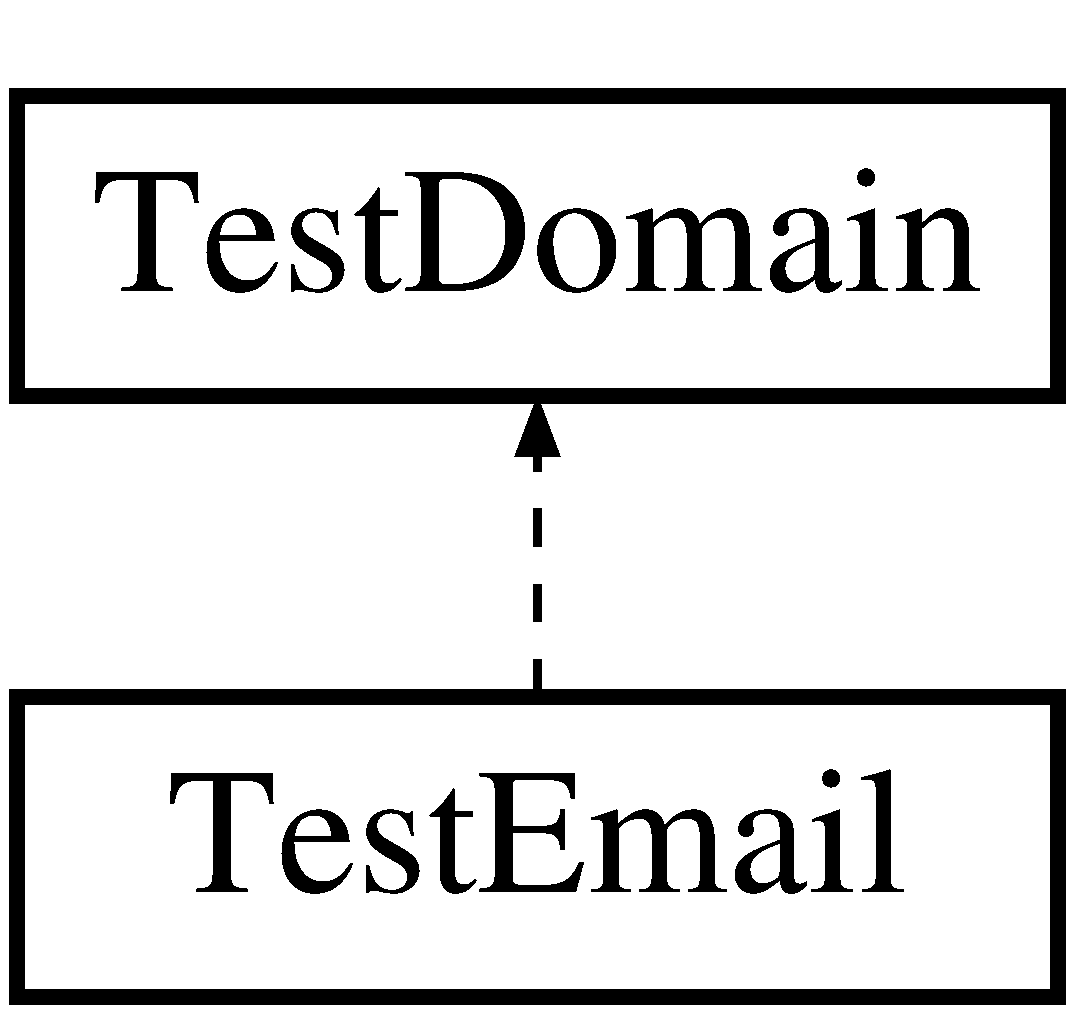
\includegraphics[height=2.000000cm]{class_test_email}
\end{center}
\end{figure}
\subsection*{Public Member Functions}
\begin{DoxyCompactItemize}
\item 
void \hyperlink{class_test_email_a55b1f52af1f5b8672c9668652384578f}{verify} ()
\item 
\hyperlink{class_test_email_a758c46261eb6b1d0570e017b95d79bd4}{Test\+Email} ()
\item 
\hyperlink{class_test_email_ad1019728841de85fb998a46aa974d9e6}{$\sim$\+Test\+Email} ()
\end{DoxyCompactItemize}
\subsection*{Additional Inherited Members}


\subsection{Constructor \& Destructor Documentation}
\mbox{\Hypertarget{class_test_email_a758c46261eb6b1d0570e017b95d79bd4}\label{class_test_email_a758c46261eb6b1d0570e017b95d79bd4}} 
\index{Test\+Email@{Test\+Email}!Test\+Email@{Test\+Email}}
\index{Test\+Email@{Test\+Email}!Test\+Email@{Test\+Email}}
\subsubsection{\texorpdfstring{Test\+Email()}{TestEmail()}}
{\footnotesize\ttfamily Test\+Email\+::\+Test\+Email (\begin{DoxyParamCaption}{ }\end{DoxyParamCaption})}

A public constructor \mbox{\Hypertarget{class_test_email_ad1019728841de85fb998a46aa974d9e6}\label{class_test_email_ad1019728841de85fb998a46aa974d9e6}} 
\index{Test\+Email@{Test\+Email}!````~Test\+Email@{$\sim$\+Test\+Email}}
\index{````~Test\+Email@{$\sim$\+Test\+Email}!Test\+Email@{Test\+Email}}
\subsubsection{\texorpdfstring{$\sim$\+Test\+Email()}{~TestEmail()}}
{\footnotesize\ttfamily Test\+Email\+::$\sim$\+Test\+Email (\begin{DoxyParamCaption}{ }\end{DoxyParamCaption})}

A public destructor 

\subsection{Member Function Documentation}
\mbox{\Hypertarget{class_test_email_a55b1f52af1f5b8672c9668652384578f}\label{class_test_email_a55b1f52af1f5b8672c9668652384578f}} 
\index{Test\+Email@{Test\+Email}!verify@{verify}}
\index{verify@{verify}!Test\+Email@{Test\+Email}}
\subsubsection{\texorpdfstring{verify()}{verify()}}
{\footnotesize\ttfamily void Test\+Email\+::verify (\begin{DoxyParamCaption}{ }\end{DoxyParamCaption})}

A public method Call the test methods with the expected values 

The documentation for this class was generated from the following files\+:\begin{DoxyCompactItemize}
\item 
\hyperlink{test__domains_8hpp}{test\+\_\+domains.\+hpp}\item 
\hyperlink{test__domains_8cpp}{test\+\_\+domains.\+cpp}\end{DoxyCompactItemize}

\hypertarget{class_test_name}{}\section{Test\+Name Class Reference}
\label{class_test_name}\index{Test\+Name@{Test\+Name}}


{\ttfamily \#include $<$test\+\_\+domains.\+hpp$>$}

Inheritance diagram for Test\+Name\+:\begin{figure}[H]
\begin{center}
\leavevmode
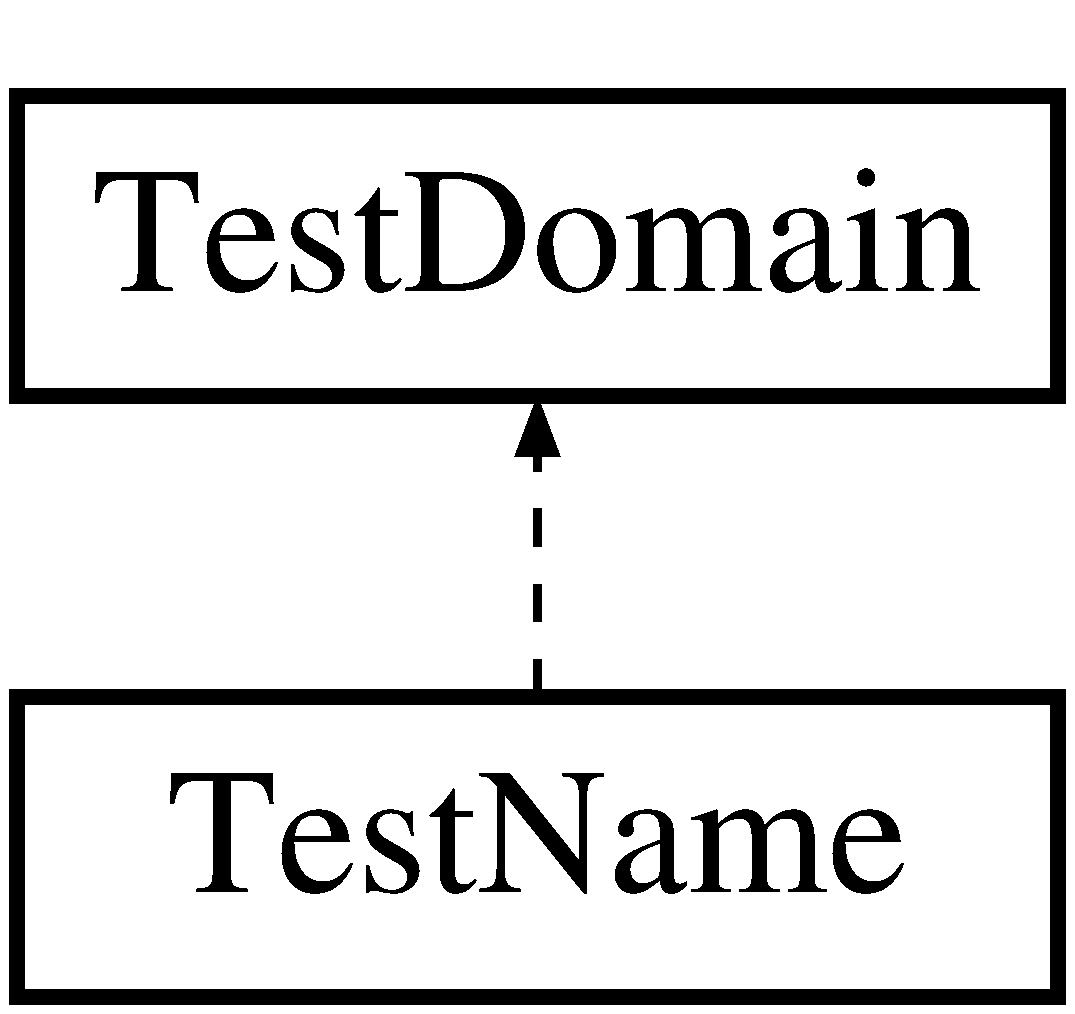
\includegraphics[height=2.000000cm]{class_test_name}
\end{center}
\end{figure}
\subsection*{Public Member Functions}
\begin{DoxyCompactItemize}
\item 
void \hyperlink{class_test_name_a578481758db2b6506d86ea8208208cfe}{verify} ()
\item 
\hyperlink{class_test_name_aebe1cb3955150d92fce4a8abec1b0d86}{Test\+Name} ()
\item 
\hyperlink{class_test_name_afc5241e6c7d586d2bc8f4d56e86431e8}{$\sim$\+Test\+Name} ()
\end{DoxyCompactItemize}
\subsection*{Additional Inherited Members}


\subsection{Constructor \& Destructor Documentation}
\mbox{\Hypertarget{class_test_name_aebe1cb3955150d92fce4a8abec1b0d86}\label{class_test_name_aebe1cb3955150d92fce4a8abec1b0d86}} 
\index{Test\+Name@{Test\+Name}!Test\+Name@{Test\+Name}}
\index{Test\+Name@{Test\+Name}!Test\+Name@{Test\+Name}}
\subsubsection{\texorpdfstring{Test\+Name()}{TestName()}}
{\footnotesize\ttfamily Test\+Name\+::\+Test\+Name (\begin{DoxyParamCaption}{ }\end{DoxyParamCaption})}

A public constructor \mbox{\Hypertarget{class_test_name_afc5241e6c7d586d2bc8f4d56e86431e8}\label{class_test_name_afc5241e6c7d586d2bc8f4d56e86431e8}} 
\index{Test\+Name@{Test\+Name}!````~Test\+Name@{$\sim$\+Test\+Name}}
\index{````~Test\+Name@{$\sim$\+Test\+Name}!Test\+Name@{Test\+Name}}
\subsubsection{\texorpdfstring{$\sim$\+Test\+Name()}{~TestName()}}
{\footnotesize\ttfamily Test\+Name\+::$\sim$\+Test\+Name (\begin{DoxyParamCaption}{ }\end{DoxyParamCaption})}

A public destructor 

\subsection{Member Function Documentation}
\mbox{\Hypertarget{class_test_name_a578481758db2b6506d86ea8208208cfe}\label{class_test_name_a578481758db2b6506d86ea8208208cfe}} 
\index{Test\+Name@{Test\+Name}!verify@{verify}}
\index{verify@{verify}!Test\+Name@{Test\+Name}}
\subsubsection{\texorpdfstring{verify()}{verify()}}
{\footnotesize\ttfamily void Test\+Name\+::verify (\begin{DoxyParamCaption}{ }\end{DoxyParamCaption})}

A public method Call the test methods with the expected values 

The documentation for this class was generated from the following files\+:\begin{DoxyCompactItemize}
\item 
\hyperlink{test__domains_8hpp}{test\+\_\+domains.\+hpp}\item 
\hyperlink{test__domains_8cpp}{test\+\_\+domains.\+cpp}\end{DoxyCompactItemize}

\hypertarget{class_test_password}{}\section{Test\+Password Class Reference}
\label{class_test_password}\index{Test\+Password@{Test\+Password}}


{\ttfamily \#include $<$test\+\_\+domains.\+hpp$>$}

Inheritance diagram for Test\+Password\+:\begin{figure}[H]
\begin{center}
\leavevmode
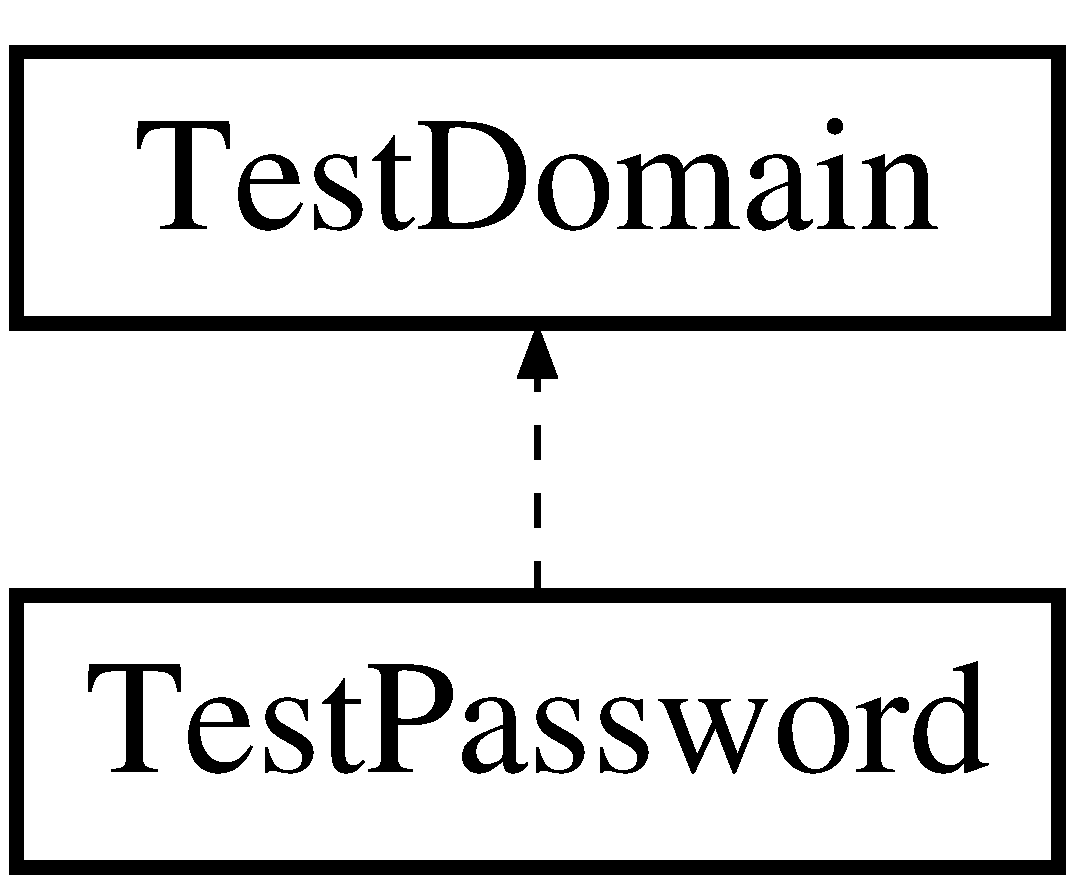
\includegraphics[height=2.000000cm]{class_test_password}
\end{center}
\end{figure}
\subsection*{Public Member Functions}
\begin{DoxyCompactItemize}
\item 
void \hyperlink{class_test_password_ac1b1f3a83e7e6b76b635a0e09004c7b6}{verify} ()
\item 
\hyperlink{class_test_password_ac69097f5ca9cf4b1684268614b7dacd2}{Test\+Password} ()
\item 
\hyperlink{class_test_password_a944afaaae5f53c83d3060f93c2f4f474}{$\sim$\+Test\+Password} ()
\end{DoxyCompactItemize}
\subsection*{Additional Inherited Members}


\subsection{Constructor \& Destructor Documentation}
\mbox{\Hypertarget{class_test_password_ac69097f5ca9cf4b1684268614b7dacd2}\label{class_test_password_ac69097f5ca9cf4b1684268614b7dacd2}} 
\index{Test\+Password@{Test\+Password}!Test\+Password@{Test\+Password}}
\index{Test\+Password@{Test\+Password}!Test\+Password@{Test\+Password}}
\subsubsection{\texorpdfstring{Test\+Password()}{TestPassword()}}
{\footnotesize\ttfamily Test\+Password\+::\+Test\+Password (\begin{DoxyParamCaption}{ }\end{DoxyParamCaption})}

A public constructor \mbox{\Hypertarget{class_test_password_a944afaaae5f53c83d3060f93c2f4f474}\label{class_test_password_a944afaaae5f53c83d3060f93c2f4f474}} 
\index{Test\+Password@{Test\+Password}!````~Test\+Password@{$\sim$\+Test\+Password}}
\index{````~Test\+Password@{$\sim$\+Test\+Password}!Test\+Password@{Test\+Password}}
\subsubsection{\texorpdfstring{$\sim$\+Test\+Password()}{~TestPassword()}}
{\footnotesize\ttfamily Test\+Password\+::$\sim$\+Test\+Password (\begin{DoxyParamCaption}{ }\end{DoxyParamCaption})}

A public destructor 

\subsection{Member Function Documentation}
\mbox{\Hypertarget{class_test_password_ac1b1f3a83e7e6b76b635a0e09004c7b6}\label{class_test_password_ac1b1f3a83e7e6b76b635a0e09004c7b6}} 
\index{Test\+Password@{Test\+Password}!verify@{verify}}
\index{verify@{verify}!Test\+Password@{Test\+Password}}
\subsubsection{\texorpdfstring{verify()}{verify()}}
{\footnotesize\ttfamily void Test\+Password\+::verify (\begin{DoxyParamCaption}{ }\end{DoxyParamCaption})}

A public method Call the test methods with the expected values 

The documentation for this class was generated from the following files\+:\begin{DoxyCompactItemize}
\item 
\hyperlink{test__domains_8hpp}{test\+\_\+domains.\+hpp}\item 
\hyperlink{test__domains_8cpp}{test\+\_\+domains.\+cpp}\end{DoxyCompactItemize}

\hypertarget{class_test_post}{}\section{Test\+Post Class Reference}
\label{class_test_post}\index{Test\+Post@{Test\+Post}}


{\ttfamily \#include $<$test\+\_\+entities.\+hpp$>$}

\subsection*{Public Member Functions}
\begin{DoxyCompactItemize}
\item 
\hyperlink{class_test_post_a6dc370335c037f5768b98c8dc8addd22}{Test\+Post} ()
\item 
\hyperlink{class_test_post_a082f87fdb7c565b5c670be7f40ea516b}{$\sim$\+Test\+Post} ()
\item 
void \hyperlink{class_test_post_a8e4d52190e6be295d251dfc348591b92}{verify} ()
\end{DoxyCompactItemize}


\subsection{Constructor \& Destructor Documentation}
\mbox{\Hypertarget{class_test_post_a6dc370335c037f5768b98c8dc8addd22}\label{class_test_post_a6dc370335c037f5768b98c8dc8addd22}} 
\index{Test\+Post@{Test\+Post}!Test\+Post@{Test\+Post}}
\index{Test\+Post@{Test\+Post}!Test\+Post@{Test\+Post}}
\subsubsection{\texorpdfstring{Test\+Post()}{TestPost()}}
{\footnotesize\ttfamily Test\+Post\+::\+Test\+Post (\begin{DoxyParamCaption}{ }\end{DoxyParamCaption})}

A public constructor \mbox{\Hypertarget{class_test_post_a082f87fdb7c565b5c670be7f40ea516b}\label{class_test_post_a082f87fdb7c565b5c670be7f40ea516b}} 
\index{Test\+Post@{Test\+Post}!````~Test\+Post@{$\sim$\+Test\+Post}}
\index{````~Test\+Post@{$\sim$\+Test\+Post}!Test\+Post@{Test\+Post}}
\subsubsection{\texorpdfstring{$\sim$\+Test\+Post()}{~TestPost()}}
{\footnotesize\ttfamily Test\+Post\+::$\sim$\+Test\+Post (\begin{DoxyParamCaption}{ }\end{DoxyParamCaption})}

A public destructor 

\subsection{Member Function Documentation}
\mbox{\Hypertarget{class_test_post_a8e4d52190e6be295d251dfc348591b92}\label{class_test_post_a8e4d52190e6be295d251dfc348591b92}} 
\index{Test\+Post@{Test\+Post}!verify@{verify}}
\index{verify@{verify}!Test\+Post@{Test\+Post}}
\subsubsection{\texorpdfstring{verify()}{verify()}}
{\footnotesize\ttfamily void Test\+Post\+::verify (\begin{DoxyParamCaption}{ }\end{DoxyParamCaption})}

A public method Call the test methods with the expected values A public method Call the test methods with the expected values 

The documentation for this class was generated from the following files\+:\begin{DoxyCompactItemize}
\item 
\hyperlink{test__entities_8hpp}{test\+\_\+entities.\+hpp}\item 
\hyperlink{test__entities_8cpp}{test\+\_\+entities.\+cpp}\end{DoxyCompactItemize}

\hypertarget{class_test_text}{}\section{Test\+Text Class Reference}
\label{class_test_text}\index{Test\+Text@{Test\+Text}}


{\ttfamily \#include $<$test\+\_\+domains.\+hpp$>$}

Inheritance diagram for Test\+Text\+:\begin{figure}[H]
\begin{center}
\leavevmode
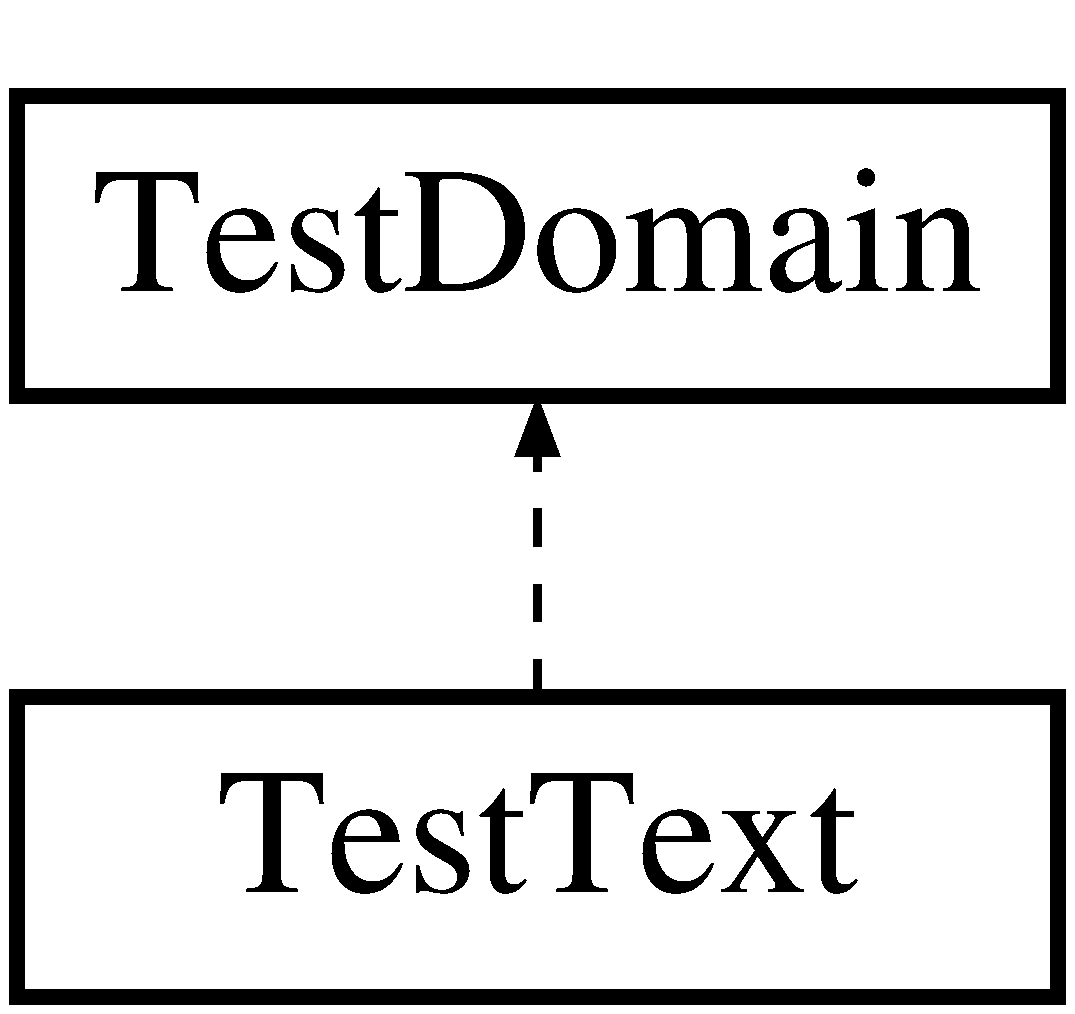
\includegraphics[height=2.000000cm]{class_test_text}
\end{center}
\end{figure}
\subsection*{Public Member Functions}
\begin{DoxyCompactItemize}
\item 
void \hyperlink{class_test_text_a31dc2a3f90d77c2db5c0278e7233f3b0}{verify} ()
\item 
\hyperlink{class_test_text_aea03a9211d87d91e33b56a46cd62a2d1}{Test\+Text} ()
\item 
\hyperlink{class_test_text_a6c7fc1f46cab52437b3d77cd7d593d40}{$\sim$\+Test\+Text} ()
\end{DoxyCompactItemize}
\subsection*{Additional Inherited Members}


\subsection{Constructor \& Destructor Documentation}
\mbox{\Hypertarget{class_test_text_aea03a9211d87d91e33b56a46cd62a2d1}\label{class_test_text_aea03a9211d87d91e33b56a46cd62a2d1}} 
\index{Test\+Text@{Test\+Text}!Test\+Text@{Test\+Text}}
\index{Test\+Text@{Test\+Text}!Test\+Text@{Test\+Text}}
\subsubsection{\texorpdfstring{Test\+Text()}{TestText()}}
{\footnotesize\ttfamily Test\+Text\+::\+Test\+Text (\begin{DoxyParamCaption}{ }\end{DoxyParamCaption})}

A public constructor \mbox{\Hypertarget{class_test_text_a6c7fc1f46cab52437b3d77cd7d593d40}\label{class_test_text_a6c7fc1f46cab52437b3d77cd7d593d40}} 
\index{Test\+Text@{Test\+Text}!````~Test\+Text@{$\sim$\+Test\+Text}}
\index{````~Test\+Text@{$\sim$\+Test\+Text}!Test\+Text@{Test\+Text}}
\subsubsection{\texorpdfstring{$\sim$\+Test\+Text()}{~TestText()}}
{\footnotesize\ttfamily Test\+Text\+::$\sim$\+Test\+Text (\begin{DoxyParamCaption}{ }\end{DoxyParamCaption})}

A public destructor 

\subsection{Member Function Documentation}
\mbox{\Hypertarget{class_test_text_a31dc2a3f90d77c2db5c0278e7233f3b0}\label{class_test_text_a31dc2a3f90d77c2db5c0278e7233f3b0}} 
\index{Test\+Text@{Test\+Text}!verify@{verify}}
\index{verify@{verify}!Test\+Text@{Test\+Text}}
\subsubsection{\texorpdfstring{verify()}{verify()}}
{\footnotesize\ttfamily void Test\+Text\+::verify (\begin{DoxyParamCaption}{ }\end{DoxyParamCaption})}

A public method Call the test methods with the expected values 

The documentation for this class was generated from the following files\+:\begin{DoxyCompactItemize}
\item 
\hyperlink{test__domains_8hpp}{test\+\_\+domains.\+hpp}\item 
\hyperlink{test__domains_8cpp}{test\+\_\+domains.\+cpp}\end{DoxyCompactItemize}

\hypertarget{class_test_user}{}\section{Test\+User Class Reference}
\label{class_test_user}\index{Test\+User@{Test\+User}}


{\ttfamily \#include $<$test\+\_\+entities.\+hpp$>$}

\subsection*{Public Member Functions}
\begin{DoxyCompactItemize}
\item 
\hyperlink{class_test_user_a354f63b1854bd20ce4f035379d873405}{Test\+User} ()
\item 
\hyperlink{class_test_user_a08bc61c08805c9fc8f1fbc33dfc84d21}{$\sim$\+Test\+User} ()
\item 
void \hyperlink{class_test_user_a56b28bed0e29a52c29104693e6fa04bf}{verify} ()
\end{DoxyCompactItemize}


\subsection{Constructor \& Destructor Documentation}
\mbox{\Hypertarget{class_test_user_a354f63b1854bd20ce4f035379d873405}\label{class_test_user_a354f63b1854bd20ce4f035379d873405}} 
\index{Test\+User@{Test\+User}!Test\+User@{Test\+User}}
\index{Test\+User@{Test\+User}!Test\+User@{Test\+User}}
\subsubsection{\texorpdfstring{Test\+User()}{TestUser()}}
{\footnotesize\ttfamily Test\+User\+::\+Test\+User (\begin{DoxyParamCaption}{ }\end{DoxyParamCaption})}

A public constructor \mbox{\Hypertarget{class_test_user_a08bc61c08805c9fc8f1fbc33dfc84d21}\label{class_test_user_a08bc61c08805c9fc8f1fbc33dfc84d21}} 
\index{Test\+User@{Test\+User}!````~Test\+User@{$\sim$\+Test\+User}}
\index{````~Test\+User@{$\sim$\+Test\+User}!Test\+User@{Test\+User}}
\subsubsection{\texorpdfstring{$\sim$\+Test\+User()}{~TestUser()}}
{\footnotesize\ttfamily Test\+User\+::$\sim$\+Test\+User (\begin{DoxyParamCaption}{ }\end{DoxyParamCaption})}

A public destructor 

\subsection{Member Function Documentation}
\mbox{\Hypertarget{class_test_user_a56b28bed0e29a52c29104693e6fa04bf}\label{class_test_user_a56b28bed0e29a52c29104693e6fa04bf}} 
\index{Test\+User@{Test\+User}!verify@{verify}}
\index{verify@{verify}!Test\+User@{Test\+User}}
\subsubsection{\texorpdfstring{verify()}{verify()}}
{\footnotesize\ttfamily void Test\+User\+::verify (\begin{DoxyParamCaption}{ }\end{DoxyParamCaption})}

A public method Call the test methods with the expected values 

The documentation for this class was generated from the following files\+:\begin{DoxyCompactItemize}
\item 
\hyperlink{test__entities_8hpp}{test\+\_\+entities.\+hpp}\item 
\hyperlink{test__entities_8cpp}{test\+\_\+entities.\+cpp}\end{DoxyCompactItemize}

\hypertarget{class_text}{}\section{Text Class Reference}
\label{class_text}\index{Text@{Text}}


{\ttfamily \#include $<$domains.\+hpp$>$}

Inheritance diagram for Text\+:\begin{figure}[H]
\begin{center}
\leavevmode
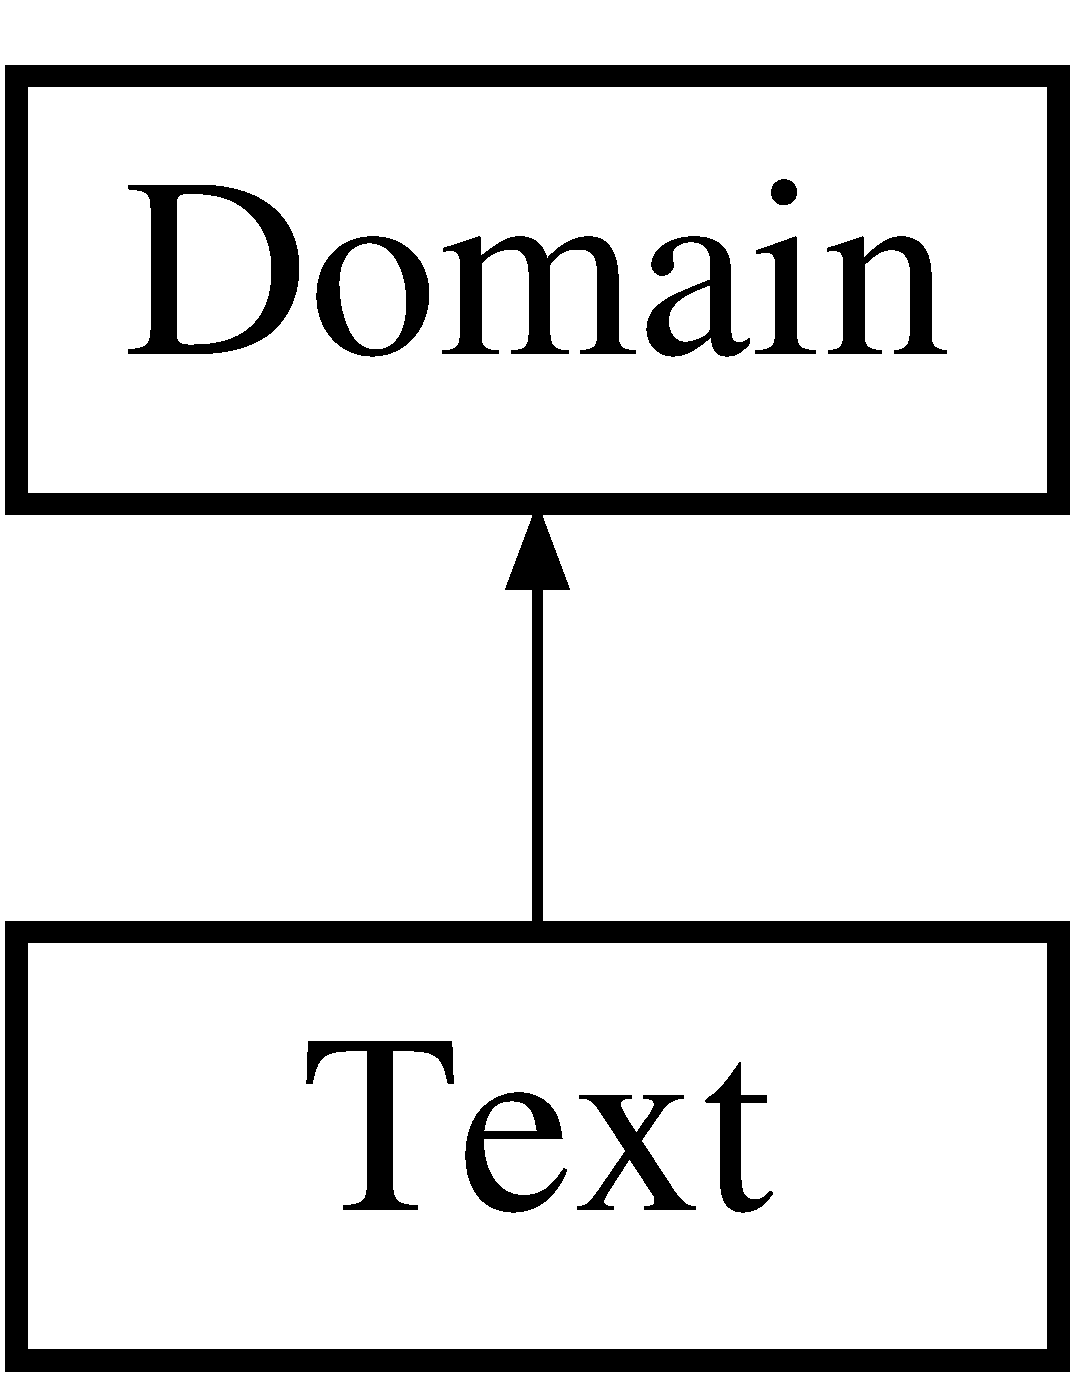
\includegraphics[height=2.000000cm]{class_text}
\end{center}
\end{figure}
\subsection*{Public Member Functions}
\begin{DoxyCompactItemize}
\item 
\hyperlink{class_text_ab3e26143fccc52699bcc5149cae852bc}{Text} ()
\item 
\hyperlink{class_text_a2d49e5c280e205125b149f7777ae30c7}{$\sim$\+Text} ()
\end{DoxyCompactItemize}
\subsection*{Additional Inherited Members}


\subsection{Detailed Description}
A class \hyperlink{class_text}{Text}. Inherit of class \hyperlink{class_domain}{Domain}. Valid the text. Verify if the text has a size less than 50 caracters. 

\subsection{Constructor \& Destructor Documentation}
\mbox{\Hypertarget{class_text_ab3e26143fccc52699bcc5149cae852bc}\label{class_text_ab3e26143fccc52699bcc5149cae852bc}} 
\index{Text@{Text}!Text@{Text}}
\index{Text@{Text}!Text@{Text}}
\subsubsection{\texorpdfstring{Text()}{Text()}}
{\footnotesize\ttfamily Text\+::\+Text (\begin{DoxyParamCaption}{ }\end{DoxyParamCaption})}

A public constructor. \mbox{\Hypertarget{class_text_a2d49e5c280e205125b149f7777ae30c7}\label{class_text_a2d49e5c280e205125b149f7777ae30c7}} 
\index{Text@{Text}!````~Text@{$\sim$\+Text}}
\index{````~Text@{$\sim$\+Text}!Text@{Text}}
\subsubsection{\texorpdfstring{$\sim$\+Text()}{~Text()}}
{\footnotesize\ttfamily Text\+::$\sim$\+Text (\begin{DoxyParamCaption}{ }\end{DoxyParamCaption})}

A public destructor. 

The documentation for this class was generated from the following files\+:\begin{DoxyCompactItemize}
\item 
\hyperlink{domains_8hpp}{domains.\+hpp}\item 
\hyperlink{domains_8cpp}{domains.\+cpp}\end{DoxyCompactItemize}

\hypertarget{class_user}{}\section{User Class Reference}
\label{class_user}\index{User@{User}}


{\ttfamily \#include $<$entities.\+hpp$>$}

\subsection*{Public Member Functions}
\begin{DoxyCompactItemize}
\item 
\hyperlink{class_user_a4a0137053e591fbb79d9057dd7d2283d}{User} ()
\item 
\hyperlink{class_user_ac00b72ad64eb4149f7b21b9f5468c2b2}{$\sim$\+User} ()
\item 
void \hyperlink{class_user_a0ecc593131bdfb1f17364ffe033d7094}{set} (\hyperlink{class_name}{Name}, \hyperlink{class_email}{Email}, \hyperlink{class_password}{Password})
\item 
\hyperlink{class_name}{Name} \hyperlink{class_user_af992bab722091aafb2024d4eacf80c59}{get\+\_\+name} ()  throw (invalid\+\_\+argument)
\item 
void \hyperlink{class_user_ad633c8904f8955905275932b19f283cf}{check\+\_\+user} (\hyperlink{class_email}{Email}, \hyperlink{class_password}{Password})  throw (invalid\+\_\+argument)
\end{DoxyCompactItemize}


\subsection{Constructor \& Destructor Documentation}
\mbox{\Hypertarget{class_user_a4a0137053e591fbb79d9057dd7d2283d}\label{class_user_a4a0137053e591fbb79d9057dd7d2283d}} 
\index{User@{User}!User@{User}}
\index{User@{User}!User@{User}}
\subsubsection{\texorpdfstring{User()}{User()}}
{\footnotesize\ttfamily User\+::\+User (\begin{DoxyParamCaption}{ }\end{DoxyParamCaption})}

A public constructor. \mbox{\Hypertarget{class_user_ac00b72ad64eb4149f7b21b9f5468c2b2}\label{class_user_ac00b72ad64eb4149f7b21b9f5468c2b2}} 
\index{User@{User}!````~User@{$\sim$\+User}}
\index{````~User@{$\sim$\+User}!User@{User}}
\subsubsection{\texorpdfstring{$\sim$\+User()}{~User()}}
{\footnotesize\ttfamily User\+::$\sim$\+User (\begin{DoxyParamCaption}{ }\end{DoxyParamCaption})}

A public destructor. 

\subsection{Member Function Documentation}
\mbox{\Hypertarget{class_user_ad633c8904f8955905275932b19f283cf}\label{class_user_ad633c8904f8955905275932b19f283cf}} 
\index{User@{User}!check\+\_\+user@{check\+\_\+user}}
\index{check\+\_\+user@{check\+\_\+user}!User@{User}}
\subsubsection{\texorpdfstring{check\+\_\+user()}{check\_user()}}
{\footnotesize\ttfamily void User\+::check\+\_\+user (\begin{DoxyParamCaption}\item[{\hyperlink{class_email}{Email}}]{email,  }\item[{\hyperlink{class_password}{Password}}]{password }\end{DoxyParamCaption}) throw  invalid\+\_\+argument) }

A public method. Check if the email and password given correspond to a real \hyperlink{class_user}{User}. T\+O\+DO\+: Need refactoring! \mbox{\Hypertarget{class_user_af992bab722091aafb2024d4eacf80c59}\label{class_user_af992bab722091aafb2024d4eacf80c59}} 
\index{User@{User}!get\+\_\+name@{get\+\_\+name}}
\index{get\+\_\+name@{get\+\_\+name}!User@{User}}
\subsubsection{\texorpdfstring{get\+\_\+name()}{get\_name()}}
{\footnotesize\ttfamily \hyperlink{class_name}{Name} User\+::get\+\_\+name (\begin{DoxyParamCaption}{ }\end{DoxyParamCaption}) throw  invalid\+\_\+argument) }

A public method \begin{DoxyReturn}{Returns}
Value of the \hyperlink{class_name}{Name} of the \hyperlink{class_user}{User}. 
\end{DoxyReturn}
\mbox{\Hypertarget{class_user_a0ecc593131bdfb1f17364ffe033d7094}\label{class_user_a0ecc593131bdfb1f17364ffe033d7094}} 
\index{User@{User}!set@{set}}
\index{set@{set}!User@{User}}
\subsubsection{\texorpdfstring{set()}{set()}}
{\footnotesize\ttfamily void User\+::set (\begin{DoxyParamCaption}\item[{\hyperlink{class_name}{Name}}]{name,  }\item[{\hyperlink{class_email}{Email}}]{email,  }\item[{\hyperlink{class_password}{Password}}]{password }\end{DoxyParamCaption})}

A public method Modify the value of the \hyperlink{class_name}{Name}, \hyperlink{class_email}{Email} and \hyperlink{class_password}{Password} of this \hyperlink{class_user}{User}. 

The documentation for this class was generated from the following files\+:\begin{DoxyCompactItemize}
\item 
\hyperlink{entities_8hpp}{entities.\+hpp}\item 
\hyperlink{entities_8cpp}{entities.\+cpp}\end{DoxyCompactItemize}

\chapter{File Documentation}
\hypertarget{domains_8cpp}{}\section{domains.\+cpp File Reference}
\label{domains_8cpp}\index{domains.\+cpp@{domains.\+cpp}}
{\ttfamily \#include \char`\"{}domains.\+hpp\char`\"{}}\newline
{\ttfamily \#include $<$bits/stdc++.\+h$>$}\newline

\hypertarget{domains_8hpp}{}\section{domains.\+hpp File Reference}
\label{domains_8hpp}\index{domains.\+hpp@{domains.\+hpp}}
{\ttfamily \#include $<$bits/stdc++.\+h$>$}\newline
\subsection*{Classes}
\begin{DoxyCompactItemize}
\item 
class \hyperlink{class_domain}{Domain}
\item 
class \hyperlink{class_name}{Name}
\item 
class \hyperlink{class_password}{Password}
\item 
class \hyperlink{class_email}{Email}
\item 
class \hyperlink{class_text}{Text}
\item 
class \hyperlink{class_avaliation}{Avaliation}
\end{DoxyCompactItemize}

\hypertarget{entities_8cpp}{}\section{entities.\+cpp File Reference}
\label{entities_8cpp}\index{entities.\+cpp@{entities.\+cpp}}
{\ttfamily \#include \char`\"{}entities.\+hpp\char`\"{}}\newline
{\ttfamily \#include $<$bits/stdc++.\+h$>$}\newline

\hypertarget{entities_8hpp}{}\section{entities.\+hpp File Reference}
\label{entities_8hpp}\index{entities.\+hpp@{entities.\+hpp}}
{\ttfamily \#include \char`\"{}domains.\+hpp\char`\"{}}\newline
{\ttfamily \#include $<$bits/stdc++.\+h$>$}\newline
\subsection*{Classes}
\begin{DoxyCompactItemize}
\item 
class \hyperlink{class_user}{User}
\item 
class \hyperlink{class_content}{Content}
\item 
class \hyperlink{class_comment}{Comment}
\item 
class \hyperlink{class_post}{Post}
\item 
class \hyperlink{class_blog}{Blog}
\end{DoxyCompactItemize}

\hypertarget{main_8cpp}{}\section{main.\+cpp File Reference}
\label{main_8cpp}\index{main.\+cpp@{main.\+cpp}}
{\ttfamily \#include $<$bits/stdc++.\+h$>$}\newline
{\ttfamily \#include \char`\"{}domains.\+hpp\char`\"{}}\newline
{\ttfamily \#include \char`\"{}test\+\_\+domains.\+hpp\char`\"{}}\newline
{\ttfamily \#include \char`\"{}test\+\_\+entities.\+hpp\char`\"{}}\newline
\subsection*{Functions}
\begin{DoxyCompactItemize}
\item 
int \hyperlink{main_8cpp_ae66f6b31b5ad750f1fe042a706a4e3d4}{main} ()
\end{DoxyCompactItemize}


\subsection{Function Documentation}
\mbox{\Hypertarget{main_8cpp_ae66f6b31b5ad750f1fe042a706a4e3d4}\label{main_8cpp_ae66f6b31b5ad750f1fe042a706a4e3d4}} 
\index{main.\+cpp@{main.\+cpp}!main@{main}}
\index{main@{main}!main.\+cpp@{main.\+cpp}}
\subsubsection{\texorpdfstring{main()}{main()}}
{\footnotesize\ttfamily int main (\begin{DoxyParamCaption}{ }\end{DoxyParamCaption})}


\hypertarget{test__domains_8cpp}{}\section{test\+\_\+domains.\+cpp File Reference}
\label{test__domains_8cpp}\index{test\+\_\+domains.\+cpp@{test\+\_\+domains.\+cpp}}
{\ttfamily \#include \char`\"{}test\+\_\+domains.\+hpp\char`\"{}}\newline
{\ttfamily \#include \char`\"{}domains.\+hpp\char`\"{}}\newline
{\ttfamily \#include $<$bits/stdc++.\+h$>$}\newline

\hypertarget{test__domains_8hpp}{}\section{test\+\_\+domains.\+hpp File Reference}
\label{test__domains_8hpp}\index{test\+\_\+domains.\+hpp@{test\+\_\+domains.\+hpp}}
{\ttfamily \#include $<$bits/stdc++.\+h$>$}\newline
{\ttfamily \#include \char`\"{}domains.\+hpp\char`\"{}}\newline
\subsection*{Classes}
\begin{DoxyCompactItemize}
\item 
class \hyperlink{class_test_domain}{Test\+Domain}
\item 
class \hyperlink{class_test_name}{Test\+Name}
\item 
class \hyperlink{class_test_password}{Test\+Password}
\item 
class \hyperlink{class_test_email}{Test\+Email}
\item 
class \hyperlink{class_test_text}{Test\+Text}
\item 
class \hyperlink{class_test_avaliation}{Test\+Avaliation}
\end{DoxyCompactItemize}

\hypertarget{test__entities_8cpp}{}\section{test\+\_\+entities.\+cpp File Reference}
\label{test__entities_8cpp}\index{test\+\_\+entities.\+cpp@{test\+\_\+entities.\+cpp}}
{\ttfamily \#include \char`\"{}test\+\_\+entities.\+hpp\char`\"{}}\newline
{\ttfamily \#include \char`\"{}domains.\+hpp\char`\"{}}\newline
{\ttfamily \#include \char`\"{}entities.\+hpp\char`\"{}}\newline
{\ttfamily \#include $<$bits/stdc++.\+h$>$}\newline

\hypertarget{test__entities_8hpp}{}\section{test\+\_\+entities.\+hpp File Reference}
\label{test__entities_8hpp}\index{test\+\_\+entities.\+hpp@{test\+\_\+entities.\+hpp}}
{\ttfamily \#include $<$bits/stdc++.\+h$>$}\newline
{\ttfamily \#include \char`\"{}domains.\+hpp\char`\"{}}\newline
\subsection*{Classes}
\begin{DoxyCompactItemize}
\item 
class \hyperlink{class_test_user}{Test\+User}
\item 
class \hyperlink{class_test_comment}{Test\+Comment}
\item 
class \hyperlink{class_test_post}{Test\+Post}
\item 
class \hyperlink{class_test_blog}{Test\+Blog}
\end{DoxyCompactItemize}

%--- End generated contents ---

% Index
\backmatter
\newpage
\phantomsection
\clearemptydoublepage
\addcontentsline{toc}{chapter}{Index}
\printindex

\end{document}
